% This is the Reed College LaTeX thesis template. Most of the work 
% for the document class was done by Sam Noble (SN), as well as this
% template. Later comments etc. by Ben Salzberg (BTS). Additional
% restructuring and APA support by Jess Youngberg (JY).
% Your comments and suggestions are more than welcome; please email
% them to cus@reed.edu
%
% See http://web.reed.edu/cis/help/latex.html for help. There are a 
% great bunch of help pages there, with notes on
% getting started, bibtex, etc. Go there and read it if you're not
% already familiar with LaTeX.
%
% Any line that starts with a percent symbol is a comment. 
% They won't show up in the document, and are useful for notes 
% to yourself and explaining commands. 
% Commenting also removes a line from the document; 
% very handy for troubleshooting problems. -BTS

% As far as I know, this follows the requirements laid out in 
% the 2002-2003 Senior Handbook. Ask a librarian to check the 
% document before binding. -SN

%%
%% Preamble
%%
% \documentclass{<something>} must begin each LaTeX document
\documentclass[12pt,twoside]{reedthesis}
% Packages are extensions to the basic LaTeX functions. Whatever you
% want to typeset, there is probably a package out there for it.
% Chemistry (chemtex), screenplays, you name it.
% Check out CTAN to see: http://www.ctan.org/
%%
\usepackage{graphicx,latexsym} 
\usepackage{amssymb,amsthm,amsmath}
\usepackage{longtable,booktabs,setspace}
\usepackage{tikz}
\usetikzlibrary{tikzmark,calc}
\usepackage{tikz-cd}
\usepackage{chemarr} %% Useful for one reaction arrow, useless if you're not a chem major
\usepackage[hyphens]{url}
\usepackage{rotating}
\usepackage{natbib}
% Comment out the natbib line above and uncomment the following two lines to use the new 
% biblatex-chicago style, for Chicago A. Also make some changes at the end where the 
% bibliography is included. 
%\usepackage{biblatex-chicago}
%\bibliography{thesis}

\newtheorem{definition}{Definition}
\newtheorem{theorem}{Theorem}
\newtheorem{assumption}{Hardness Assumption}
% \usepackage{times} % other fonts are available like times, bookman, charter, palatino

\title{Functional Encryption and Obfuscation}
\author{Sage R. Michaels}
% The month and year that you submit your FINAL draft TO THE LIBRARY (May or December)
\date{May 2018}
\division{Computer Science and Mathematics}
\advisor{Dylan McNamee}
%If you have two advisors for some reason, you can use the following
%\altadvisor{Your Other Advisor}
%%% Remember to use the correct department!
\department{Computer Science and Mathematics}
% if you're writing a thesis in an interdisciplinary major,
% uncomment the line below and change the text as appropriate.
% check the Senior Handbook if unsure.
\thedivisionof{The Established Interdisciplinary Committee for}
% if you want the approval page to say "Approved for the Committee",
% uncomment the next line
\approvedforthe{Committee}

\newcommand{\coloneqq}[0]{:=}
\newcommand{\gen}[0]{\text{Gen}}
\newcommand{\enc}[0]{\text{Enc}}
\newcommand{\dec}[0]{\text{Dec}}
\newcommand{\Z}[0]{\mathbb{Z}}

\setlength{\parskip}{0pt}
%%
%% End Preamble
%%
%% The fun begins:
\begin{document}

  \maketitle
  \frontmatter % this stuff will be roman-numbered
  \pagestyle{empty} % this removes page numbers from the frontmatter

% Acknowledgements (Acceptable American spelling) are optional
% So are Acknowledgments (proper English spelling)
    \chapter*{Acknowledgements}
	
		
	I'd like to take a moment to thank all the people who have shared in many of the great moments in my life, housemates, study buddies, friends, professors, and anyone who has torn it up on the dance-floor with me, even if your name does not appear below it does not detract from the glory of our time spent together. 
	\par I'd like to specifically, thank in no particular order, Yoel Ferdman,  Siena Ward, Yarden Refaely\footnote{aka DJ Fast Dad}, Cara Chae-Banks, Samuel ``SandBird'' Polterock, Max Vinetz, Rosa ``RoBro'' Brotherton, Alon Averbuj, Josh ``Bayz'' Biase\footnote{aka DJ Flat Soda}, and Bryant Volk\footnote{aka DJ Strong Nerd} for the beautiful friendships we have maintained in all the years we have spent apart.  	
	\par I'd also like to thank my family Sue Coles, Kiote Coles, Sierra Gomez-Saltzman, Tillie Castro, and especially Jody Saltzman and Dan Michaels for all the love over the years, without whose support none of this would have been possible.
	\par Finally, I'd like to thank my thesis advisor (and Unix mentor) Dylan McNamee for his patience, advice, pep talks, and positivity throughout this thesis process. 


% The preface is optional
% To remove it, comment it out or delete it.
    \chapter*{Abstract}
	Functional encryption is a powerful cryptographic primitive that extends the functionality of the decryption algorithm in standard encryption schemes. Currently the development of functional encryption is a rich area of cryptographic research, however much of the literature describing how functional encryption is used and constructed can be dense and unapproachable. This thesis works to make the theory behind multilinear maps, circuit obfuscation and how they are used to construct functional encryption in a way that is digestible to undergraduates. Once we have built up a theoretical understanding of functional encryption we describe a new protocol for secure online first price sealed bid auctions. Then we make use of 5Gen-C, a framework currently in development, to implement some of the first multi-input functional encryptions of binary comparison circuits (that calculates \textit{greater than}) for upto 32 by 32 bit inputs. We also use 5Gen-C to compare the efficiency of two different methods of generating comparison circuits, and find that the cascading method is more efficient for obfuscation than our recursive approach. Last we use 5Gen-C to see how functional encryption and obfuscation are currently infeasible for complex computations due to the exponential increase in setup runtime as the multilinearity of the underlying multilinear map increases.
	

    \tableofcontents
% if you want a list of tables, optional
%    \listoftables
% if you want a list of figures, also optional
 %   \listoffigures
    
 
  \mainmatter % here the regular arabic numbering starts
  \pagestyle{fancyplain} % turns page numbering back on   
    
     \chapter*{Introduction}
         \addcontentsline{toc}{chapter}{Introduction}
	\chaptermark{Introduction}
	\markboth{Introduction}{Introduction}
	        Historically, encryption has been the cryptographic primitive that allows for two (or more) parties to exchange private information through untrusted channels. That is to say, if Alice wishes to send Bob an invitation to a party, but does not want anyone else to see it, Alice could encrypt the invitation in such a way that only Bob could decrypt it, and then send it over to Bob. If the message is properly encrypted then Alice can sends the message by any convenient means without worrying who else might see the message, since \textit{only} Bob can make sense of it through decryption. Indeed we use this type of encryption all the time for sending emails, sms text messages, online shopping, and e-banking so long as we are using the correct apps and settings.
	        \par However, in a world where individuals store much of their data on the cloud, the method of encryption just described might be either too limiting or give away too much information. For example, suppose Alice has so many digital photos that she has to store them on Amazing Cloud Services. While Alice likes Amazing Cloud Services, she does not want them to be able to look through all her photos, so she encrypts each photo, along with their affiliated information such as location and date taken, before uploading it to the cloud. Perhaps one day Alice wants to look at all her photos taken in 2008, how should she go about getting these photos from Amazing? Since all the photos are encrypted, Amazing cannot actually look and see which photos were taken when. With the standard notion of encryption, Alice either needs to sacrifice her privacy and teach Amazing Cloud Services how to decrypt her photos so they can send her the ones from 2008, or needs to download and decrypt each photo in order to determine when it was taken; which would be difficult since her computer space and bandwidth is limited. For situations like this Alice would want to be able to come up with another way to decrypt that gives Amazing the ability to see if an encrypted photo is from 2008 or not, but nothing else. We call encryption schemes that can decrypt to functions of messages rather than just messages in their entirety, functional encryption schemes.
	        \par In order to construct functional encryption, we need another cryptographic primitive known as obfuscation. The goal of obfuscation is to take a program or circuit and make it unintelligible so that running the program on an input reveals nothing else about the input other than the output of the program. Currently, many methods of obfuscation rely on the conversion of circuits or programs into matrices and the encoding of those matrices with a data structure known as a graded encoding scheme that enables computation on encoded inputs so that only information about the final result of the computation can be learned.
	\par In standard encryption (i.e. where we can only get the full message from decryption), we expect that the recipient of a message has a secret key that allows them to fully decrypt messages. Typically these secret keys are random sequences of ones and zeros, however with functional encryption we instead send obfuscated circuits as evaluation keys. After we are convinced that functional encryption is theoretically possible, we can construct protocols that use it in new and interesting ways. There are also existing frameworks that have instantiated both functional encryption and obfuscation. The 5Gen-C framework allows us to run experiments on the efficiency of these primitives and protocols to determine the current feasibility of using them.
	\par Much of the literature that discusses the construction of functional encryption can be dense and unapproachable for an undergraduate computer science student. This thesis was written by and for undergraduates with the intention of being an approachable resource for understanding the basics of functional encryption, obfuscation, how it is constructed, and its applications. Although this work is intended to be accessible to anyone interested in reading it, at certain points of this work we will assume that the reader has a basic understanding of modern cryptographic concepts as found in \cite{Katz:2007:IMC:1206501}. We also assume that the reader is somewhat familiar with group and ring theory as would be taught in an undergraduate abstract or modern algebra course. Although these assumptions are made of the reader, we cite information rather liberally, so even a reader without these prerequisites, with some extra effort, should be able to obtain a reasonable understanding of the topics discussed in this thesis. This work draws heavily on \cite{Garg:2013} and \cite{GGH13}; and used software from Galois Inc. as described in \cite{5genc}.
    
   
    

    
    \chapter{Background}
    \section{Encryption}
    Encryption is a way to share a message so that only the intended recipient(s) of
    that message are able to read it. Historically this was done by means of obscurity, in the sense that correspondents assumed only they knew the specific method by which messages between them would be encrypted. The problem with encryption via obscurity is that as soon as a method of encryption becomes popular, it also becomes obsolete.
    \subsection{Standard Encryption}
    Now, cryptographers work to develop encryption schemes that are computationally infeasible for adversaries to break even if the method of encryption is known (this is known as Kerckhoff's Principle). To do this, encryption functions are made public but use random secret keys to conceal the message. The best keys are ones that are decently long and chosen randomly over some distribution (often uniformly), so it is infeasible for an adversary to check every possible key or guess the right key using information about communicating parties.
       \par In defining an encryption scheme we call the set of all valid keys $K$: ``the key space''; the set of all valid messages $M$: ``the message space'', and the set of all valid ciphertexts (encrypted messages) $C$: ``the cipher space''.

\begin{definition}[Standard Encryption Scheme]
     
 
 $$\text{Gen}:\mathbb{Z} \rightarrow K \times K$$
 Defined to be for $\lambda \in \mathbb{Z}$, Gen($\lambda ) \rightarrow (pk,sk)$ where $pk$ and $sk$ are random keys of length $\lambda$.
 
  $$\text{Enc}:K \times M \rightarrow C$$
Defined for key $pk\in K$ and message $m\in M$; to be Enc$(pk,m) \rightarrow c$ for some ciphertext $c\in C$
 
 $$\text{Dec}:K \times C \rightarrow M$$
 Defined for key $sk \in K$ and ciphertext $c\in C$; to be Dec$(sk,c) \rightarrow m$ for some message $m\in M$
 
 \end{definition}
 
 
\par If $sk = pk$ this is called a symmetric or private key encryption scheme meaning only the correspondents know the key and they keep it secret. If $sk \not= pk$ then this is called an asymmetric or public key encryption scheme where $sk$ is a secret key and $pk$ is a public key. In a public key encryption scheme anyone can encrypt a message since the public key is public, but only people with the secret key are able to decrypt.


\begin{definition}[Correctness]
In this setting we say an encryption scheme $\Pi$ is \textbf{correct} if for $n\in \mathbb{Z} , (sk,pk) \leftarrow$ Gen$(n)$ and $m\in M$ 

$$\text{Dec}(sk, (\text{Enc}(pk,m)) = m$$
\end{definition}

\par Suppose Alice and wants to send Bob a secret message $m$. To do this in the public key setting Bob would have to run Gen$(n) \rightarrow (pk, sk)$ and then send $pk$ to Alice. Then Alice gets $c:= $Enc$(pk,m)$ and sends $c$ over to Bob. Finally Bob gets $m':= $Dec$(sk, c)$. If the scheme is correct then $m' = m$ and Bob is able to read Alice's message. The above interaction is represented in the following diagram.

\begin{table}[ht]
  \centering
  \fbox{
  \begin{tabular}{c c c}
    Bob & & Alice \\ 
    $\gen(\lambda) \rightarrow (sk,pk)$ &&\\
    & $\xrightarrow{\quad pk \quad}$ & \\
    & & $\enc(pk,m) \rightarrow c$ \\
    & $\xleftarrow{\quad c \quad}$& \\
    $m' \coloneqq \dec(pk,c)$ && \\
  \end{tabular}
  }
   \caption{Public Key Encryption Protocol}
  \end{table}


\par We also care about the security of an encryption scheme. That is to say, we want to ensure that an encryption scheme is \textit{good} at hiding the information that we are encrypting. There are many different types of security, here we will focus on CPA-Security. Informally, we say an encryption scheme is secure against chosen plaintext attacks  (hereby CPA-Secure) if an adversary is unable to differentiate the ciphertexts from two known and distinct messages. 
\\
\\ More formally, we define CPA security with the following game: \\
\begin{definition}{CPA-Game and Security}
\par Suppose we have the following encryption scheme $($Gen,Enc,Dec$)$ with $(pk,sk) \leftarrow \text{Gen}(\lambda).$ Then for any adversary $\mathcal{A}$, we give them $pk$ and our encryption function Enc. They can then encrypt whatever messages they want, and eventually give us the messages $m_0$ and $m_1$. We then run Enc$(pk,m_b)\to c_b$ for $b$ chosen with probability $1/2$, and give $c_b \to \mathcal{A}$. After some time $\mathcal{A}$ outputs a bit $b'$. 
\par We say $\mathcal{A}$ is successful if $b=b'$ and we say an encryption scheme is CPA-Secure if no adversary is able to succeed at the CPA-Game with probability more than $1/2$.
\end{definition}


\subsection{Functional Encryption}

With standard encryption, decryption is all or nothing, either you have the secret key and can find out the message, or you do not have the secret key so you can not learn anything about the encrypted message. With functional encryption we formalize and broaden the functionality of the decryption algorithm so that it can yield specific functions of messages from ciphertext as opposed to just the entire message. We start with a definition and then formalize the scheme.
\begin{definition}[Correctness]
A Functional Encryption Scheme $\Pi$ is \textbf{correct} if for $m \in M$, some predetermined function $f$ with $M$ as its domain, and appropriate public key and \textit{evaluation} key $(PK,SK_f)\in K$ from $\Pi$'s key generation algorithm:

$$\dec(SK_f, \enc(PK,m)) = f(m) $$
\end{definition}

It is easy to see that this definition encapsulates the older definition of correctness by making $f$ the identity function $f(m) = m$, but this syntax covers many other cryptographic primitives as well like attribute based encryption (ABE) and identity based encryption (IBE). To see how these primitives are subcases of functional encryption lets formalize our idea of a functional encryption scheme. 




\begin{definition}[Functional Encryption Scheme]
Given a message space $M$, a cipher space $C$, a family of functions $\mathcal{F}$, and a key space $K$, a functional encryption scheme $\Pi$ is defined to be the following four algorithms:

$$\text{Setup}: \Z \rightarrow K \times K$$
Defined for $\lambda \in \Z$; to be Setup($\lambda) \rightarrow (PP,MSK)$, generates a public parameter and master secret key both in $K$
$$\text{Gen}: K \times \mathcal{F} \rightarrow K $$
Defined for $f \in \mathcal{F}, MSK \in K$; to be Gen$(MSK,c) \rightarrow SK_f$ which is kept secret and is the secret key associated with the functionality of $f$.

$$\enc: K \times M \rightarrow C$$
Defined: For $PP\in K$ and $m \in M;$ to be $\enc(PP,m) \rightarrow c$

$$\dec:K \times C \rightarrow M$$
Defined for $SK_f \in K$ and $c \in C;$ to be $\dec(SK_f,c) \rightarrow m'$ if the scheme is correct then $m' = f(m)$ for some previously encrypted $m\in M$ and some $f\in \mathcal{F}$.

\end{definition}



\par Suppose Alice wants to store some text files ($\{m_1,m_2,\cdots, m_n \}$) on Bob's Cloud Storage to retrieve at some later date.
 Bob, owner of Bob's Cloud Storage, has a strong dislike for cats and does not want anything stored on
  his cloud with the word ``cat'' in it. Alice and Bob contact Janet, an impartial third party, and share their desired functionalities: Alice wants to be able to fully decrypt (i.e. identity functionality), Bob wants to be able to check if the word ``cat'' is in anything stored on his server (we call this function checking for the word ``cat'' $f$). Janet runs Setup$(\lambda)\rightarrow (PP, MSK)$ and publishes the public parameter, and also runs Keygen$(MSK,id) \rightarrow SK_{id}$ and Keygen$(MSK,f) \rightarrow SK_f$. Then Janet securely sends $SK_{id}$ to Alice and $SK_{f}$ to Bob. Now Alice encrypts her text files Enc$(PP, m_1) \rightarrow c_1,$Enc$(PP,m_2) \rightarrow c_2, \cdots $,Enc$(PP, m_n) \rightarrow c_n,$ and sends $\{c_1,c_2, \cdots, c_n \}$ to Bob for storage. Bob then runs $\dec(SK_f , c_1) \rightarrow b_1 , \cdots, \dec_{SK_f}(c_n) \rightarrow b_n $ and allows storage of all $c_i$ that indicate the word ``cat'' is not being stored.  This interaction is illustrated in figure 1.1.
  
  \begin{figure}[htbp]
	% the options are h = here, t = top, b = bottom, p = page of figures.
	% you can add an exclamation mark to make it try harder, and multiple
	% options if you have an order of preference, e.g.
	% \begin{figure}[h!tbp]
	   
	       \centering
	    % DO NOT ADD A FILENAME EXTENSION TO THE GRAPHIC FILE
	   \begin{tikzcd}
\text{\large Bob} & \text{\large Janet} & \text{\large Alice} \\
{} & \text{\small Setup}(\lambda) \rightarrow (MSK,PP) \arrow[r, "PP"] \arrow[l, "PP"'] & {} \\
{} \arrow[r, "f"] & {} & {} \arrow[l, "\text{id}"'] \\
 & \text{\small KeyGen}(id,MSK) \rightarrow SK_{\text{id}} \arrow[r, "\text{secure}(SK_{\text{id}})"] & {} \\
{} & \text{\small KeyGen}(f,MSK) \rightarrow SK_{f} \arrow[l, "\text{secure}(SK_f)"'] &  \\
 &  & \text{\small Enc}(PP, m_1)\rightarrow c_1 \\[-28]
 &  & \vdots \\[-25pt]
 &  & \text{\small Enc}(PP, m_n)\rightarrow c_n \\
{} &  & {} \arrow[ll] \{c_1, \cdots, c_n \} \\
\text{\small Dec}(SK_{f}, c_1) \rightarrow b_1 &  &  \\[-28pt]
\vdots &  &  \\[-25pt]
\text{ \small Dec}(SK_{f},c_n) \rightarrow b_n &  & 
\end{tikzcd}


	     \caption{Diagram describing protocol for Alice securely storing files on Bob's cloud services using functional encryption}
	 \label{subd}
	\end{figure}

\par Since Alice has $SK_\text{id}$ if she want to access a poem that she had written and stored on Bob's server, she can request that Bob send over her data, at which point she can run Dec$(SK_\text{id}, c_p)$ on the ciphertext $c_p$ containing her poem so that she can read it in full.  Of course having to download all the data she had stored is not optimal, and neither is having to decrypt all the ciphertexts to find the poem she is looking for, but this is just a toy example for us to get a taste for using functional encryption. We will get into more detailed protocols in chapter 4.


\par It should be noted that the impartial 3rd party does not need to be fully trusted since Janet doesn't have any of Alice's ciphertexts to decrypt, but it is important that Janet is impartial since otherwise should could collude with Alice to store a Cat Encyclopedia on Bob's Servers, or could collaborate with Bob to learn more about what Alice is storing than what Alice and Bob have agreed upon. 


\par As with the standard notion of encryption, we want to be able to discuss the security of a functional encryption scheme. While we would like a functional encryption scheme to be CPA secure against eavesdroppers who do not have secret keys, we also need to be sure that parties with secret keys are unable to learn more about ciphertexts than what they learn just from  the decryption function. As before our security definition is game based, although this time we call it indistinguishability security.\\

\begin{definition}{Indistinguishability Security}
\par Let $($Setup,Gen,Enc,Dec$)$ be a functional encryption scheme and $(PP,MSK)\leftarrow$Setup$(\lambda)$. Then for an adversary $\mathcal{A}$ 
\begin{itemize}
\item We give $PP,$ Enc, and Dec to $\mathcal{A}$ who can then query for a secret key that computes $f_i$. After receiving a query for $f_i$ we run Gen$(MSK,f_i) \to SK_{f_i}$ and send $SK_{f_i}$ to $\mathcal{A}$.
\item Eventually $\mathcal{A}$ sends us two messages $m_0,m_1$ where $f_i(m_0)=f_i(m_1)$ for all functions queried so far. We then run Dec$(MSK,m_b)\to c_b$ for $b$ chosen with probability $1/2$ and send $c_b$ to $\mathcal{A}$.
\item $\mathcal{A}$ can continue to send us queries for functions $f_i$ where $f_i(m_0) = f_i(m_1)$ which we will generate and send keys for. After some time $\mathcal{A}$ outputs a bit $b'$.
\end{itemize}
\par As before we say $\mathcal{A}$ is successful if $b = b'$, and we say a functional encryption scheme is indistinguishability secure if no adversary is able to succeed with probability greater than $1/2$.
\end{definition}

\par Simply put, our security definition says that no adversary should be able to use a secret key $SK_f$ to learn anything else about a ciphertext than the output of $f$ on the encrypted message. We require that $f(m_1)=f(m_0)$ for all queries because we want individuals with secret keys to be able to functionally decrypt, but this would differentiate any two messages where $f(m_0) \not= f(m_1)$. This security definition encapsulates CPA security since if an adversary can distinguish two messages just from their ciphertext then they would be able to consistently succeed at the indistinguishability game. We will not be doing any security proofs in this work, so this is about the extent to which we will cover security definitions of functional encryption, but for further discussion on security definitions see [\cite{funcenc}].

\par Research into functional encryption is currently at early stages, later we will describe the details of how it works and where it's currently limited. Even at such an early stage cryptographic research, functional encryption has proven to be a powerful tool giving us a variety of functionalities with only small alterations of syntax such as attribute based encryption, identity based encryption , and multi-party input functional encryption [\cite{funcenc}] which we will work with later on. 

    
    

    \section{Obfuscation}
    A concern that needs to be addressed in order for us to construct functional encryption is: how can we ensure that some adversary given a secret key $SK_f$ for a function $f$ cannot alter $SK_f$ after it has been generated to reveal more information about ciphertexts than intended? 
    \par For example, suppose $f(x_1,x_2) = x_1 + x_2$, since cryptographers assume Kerckoff's principle that the way $PK_f$ is generated should be public, an adversary might be able to take advantage of the ordering of the sum in $f$ in order to learn the value of $x_1$ and $x_2$.
    \par To prevent the functionality of $SK_f$ from being altered, we want to obfuscate $f$ so that no adversary can take advantage of how $SK_f$ is generated from $f$ to alter the key's functionality. It is easy to obfuscate functions, programs, encodings, etc... but it is difficult to \textit{provably} obfuscate anything, after all defining obfuscation is not easy to conceptualize. In this section we discuss different attempts at formalizing obfuscation and in chapter 3 we will construct it.
    
    \subsection{Black Box Obfuscation}
     \par Circuit (and program) obfuscation is a cryptographic method that seeks to make a circuit unintelligible to anyone looking at only its obfuscation. The goal of black box obfuscation as defined in [\cite{vbb}] is that a circuit that has been black box obfuscated should reveal no more about its inner workings than a table of inputs and outputs for the same circuit (we call this table an Oracle).
         
     \par Let's take a moment to talk about why cryptographers would want black box obfuscation as a tool. Currently public key encryption relies on expensive computations, (for example in RSA the private keys are just inverses of public keys in some group large enough for factoring to be difficult to compute). However, private key encryption is much more efficient since it's just running some sort of permutation on the message using the secret key and then descrambling the ciphertext with the same secret key. Using black box obfuscation it would be possible to obfuscate a private key encryption function with a secret key $sk$ baked in $\mathcal{O}(\enc_{sk}(\cdot)) \rightarrow \enc(\cdot)$ where $\enc(\cdot)$ can be made public without risk of anyone learning $sk$ keeping the ability to decrypt in the hands of those who started off with the secret key. Thus Black Box Obfuscation would make efficient private key encryption into efficient public key encryption.
    
    
    
    \subsection{Indistinguishability Obfuscation}
   
   
    While Black Box Obfuscation was proved impossible in [\cite{vbb}], cryptographers weakened their definition of obfuscation to try and see what \textit{is} possible in the field of obfuscation. This led to a new notion of obfuscation called \textit{indistinguishability obfuscation}. 
    \par Before defining indistinguishability obfuscation it is worth noting that a distinguisher is any polynomial time algorithm that can differentiate two things. For example, a distinguisher for apples and oranges might look at the color of what it has been given and output  \textit{orange} if the color is orange or \textit{apple} if the color of what it has been given is red/green/yellow, however another distinguisher for apples and oranges might just flip a coin and output \textit{apple} if the coin comes up heads and \textit{orange} otherwise. Note the second distinguisher would probably not be a very good at distinguishing apples from oranges. Distinguishers are only defined on the two things that they distinguish, apples or oranges, green or blue, paper or not paper.
       \newcommand{\iO}[0]{\textit{i}\mathcal{O}}
    
    \begin{definition}{Indistinguishability Obfuscation}
    \par Given circuits $C_0,\ C_1$ where $|C_0| \approx |C_1|, C_0(x) = C_1(x)$ for all valid $x$, and an obfuscater $\iO(\cdot)$; we say that $\iO$ is an \textbf{indistinguishability obfuscater} if for all Distinguishers $\mathcal{D}$
    $$\Pr[\mathcal{D}(\iO(C_0)) = 1] -\Pr[\mathcal{D}(\iO(C_1)) = 1] \leq \text{negl}$$
    \end{definition}
    
    \par This definition can be a little confusing to understand. In short, I \textit{indistinguishability obfuscation} guarantees that two circuits with the same functionality are indistinguishable from one another once run through an indistinguishability obfuscater. 
    \par What can be more confusing is why this would be useful since we require the two circuits to be functionally the same. The most simple usage is in removing watermarks from programs. Suppose Dan buys a fancy piece of software called Macrosoft Word for his company. Macrosoft is worried about their software being pirated so they put a watermark in Dan's copy of Macrosoft Word that does not change the functionality of his copy of the program, but indicates that it is Dan's copy. Suppose Dan wants to make Macrosoft Word free for everyone and decides to post it on a torrenting website. If Dan posts his copy as is, Macrosoft and their copyright lawyers will be able to see that it was Dan who illegally shared his copy of their software. Instead, if Dan first runs his copy of Macrosoft word through an indistinguishability obfuscater before uploading it, Macrosoft and their lawyers will be unable to tell if it was Dan's copy that was posted, or another customer's.
    \par This might seem like a weak definition, but indistinguishability obfuscation has become a powerful cryptographic tool, and has proven to be the best possible obfuscation, in [\cite{Goldwasser:2007:BO:1760749.1760765}]. As a result cryptographers often treat indistinguishability obfuscation the same as Black Box Obfuscation. While this could lead to issues in the future and there is lots of room for work to be done in quantifying degrees of obfuscation, we will fall back on the assumption that the best possible obfuscation is good enough for our purposes.
    \par In cryptography, a common way to hide information is by randomization, yet to implement obfuscation we need a way of randomizing computations so that they cannot be reverse engineered since the order of computation could be utilized by a distinguisher to differentiate two circuits with the same functionality. To do this we utilize a data  structure called a graded encoding scheme which relies heavily on multilinear maps. 
    
    
    \section{Bilinear Maps}
    
    Lastly we give a brief introduction to bilinear maps, and the properties they have which we will generalize to multilinear maps in chapter 2. 
    
    \subsection{Definition}
    
    \begin{definition}{Bilinear Maps}
    \par Let $G_1,G_2,G_3$ be cyclic groups of prime order $p$. Then we say a map $e:G_1 \times G_2 \rightarrow G_3$ is bilinear if
    
    \begin{enumerate}
    \item For all $g_1 \in G_1, g_2\in G_2,$ and $ \alpha \in \Z_p, \; e(\alpha\cdot g_1,g_2) =e( g_1,\alpha\cdot g_2) = \alpha\cdot e(g_1,g_2) $
    \item For generators $g_1\in G_1, \; g_2 \in G_2, \;$ and $g_3 \in G_3,\; e(g_1,g_2) = g_3$     \end{enumerate}    
    \end{definition}
    
    \subsection{Intuition}
    \newcommand{\params}[0]{\textbf{params}}
    The most accessible example of Bilinear Map is in Tripartite Diffie-Hellman Key Exchange. Here the Bilinear Map $e:G_1 \times G_1 \rightarrow G_2$ is defined $e(g_1^a,g_1^b) \rightarrow g_2^{a\cdot b}$ for generators $g_1\in G_1$ and $g_2 \in G_2$. We can think of $a,b$ as secrets and $g_1^a,g_1^b$ as their encodings in $g_1$. Using the map $e$ we can multiply secrets and by multiplying encodings $g^a\cdot g^b = g^{a+b}$ we can also add secrets in the clear without revealing their value.
\par Suppose Alice, Bob and Carol wish to agree upon a single secret key for the three of them. To do so Alice would run an instance generation function that outputs a description of the group $G_1$, a generator $g_1$ and a bilinear map $e$ as we defined above. Then she would choose a secret $a \in \Z_p$ and broadcast $(e \in \params, g_1, pk_a := g_1^a)$. Then Bob would choose $b\in \Z_p$ and broadcast $pk_b := g_1^b$ and Alice would do the same broadcasting $pk_c := g_1^c$. For each party to learn the secret key they would need to run:
\begin{align*}
\text{Alice:} & \; e(pk_b,pk_c)^a = e(g_1^b,g_1^c)^a = ( g_2^{b\cdot c} )^a = g_2^{a\cdot b \cdot c} = sk\\
\text{Bob:} &\; e(pk_a,pk_c)^b = g_2^{a \cdot b \cdot c} = sk \\
\text{Carol:}& \; e(pk_a,pk_b)^c = g_2^{a \cdot b \cdot c} = sk
\end{align*}

\par The important thing to understand is that this bilinear map makes it possible for three parties to share a secret without risk of an eavesdropper also being able to know the secret. 

%To generalize, a $k$-multilinear map allows us to encode $k$ secrets easily, so if each party involved in the exchange knows a secret this allows for $k+1$ non interactive key exchange.

    \subsection{Hardness Assumption}
    
    In order to talk about how secure it is to run protocols that use bilinear maps (such as Alice, Bob, and Carol's key exchange) we need to formalize what the adversary would need to be able to do in order to compromise security. We call these formalizations \textit{hardness assumptions}.
    \par First we define the following problems.
    
    \begin{definition}{Bilinear Computational Diffie-Hellman Problem}
    \par Let $G_1,G_2$ be cyclic groups of prime order $p$ and $e:G_1 \times G_1 \to G_2$ be a bilinear map. For $a,b,c,\in \Z_p$ chosen uniformly and $g_1,g_2$ generators of $G_1,G_2$ respectively. The Computational Diffie-Hellman problem is: given $e,g_1,g_1^a,g_1^b$ and ,$g_1^c$; compute $$e(g_1,g_1^{a\cdot b \cdot c}) = g_2^{a\cdot b \cdot c}$$
    \end{definition}
    
    The computational Diffie-Hellman problem might seem a bit confusing, but it is pretty much just a formalization of what we realized after discussing tripartite key exchange: multiplying two secrets is easy using bilinear maps, but that multiplying by a third secret is difficult. Thus we have
    \begin{assumption}{Bilinear CDD hardness assumption}
    \par The bilinear computational Diffie-Hellman problem is hard.
        \end{assumption}
        
        \par Another hardness assumption that we need to make is the bilinear discrete logarithm problem defined below.
       
    \begin{definition}{Bilinear Discrete Logarithm}
    Let $G_1,G_2$ be cyclic groups of prime order $p$ and $e:G_1 \times G_1 \to G_2$ be a bilinear map. For $a \in \Z_p$ chosen uniformly, and generators $g_1,g_2$ of $G_1,G_2$ respectively, the bilinear discrete logarithm problem is: given $g_1,g_1^\alpha, G_1, G_2,$ and $e$ find $\alpha$.
    \end{definition}
    
    Note that while the above problem may seem easy, the encoding $g_1^\alpha = g $ just looks like some element of $G_1$, and since $g_1$ is a generator of $G_1$, \textit{any} element of $G_1$ can be written as $g_1^\beta \; \forall \beta \in \Z_p$. We want it to be difficult to get a secret out of its encoding, so we also rely on the following assumption.
    
    \begin{assumption}{Bilinear DL hardness assumption}
    \par The bilinear discrete logarithm problem is hard
    \end{assumption}
   
    
   \par There are arguments about if these are \textit{good} assumptions to be making, but these arguments are outside the scope of this thesis. It is enough for us that so far cryptographers and mathematicians have been unable to give efficient solutions to solving these problems in general cases.
    
    
    \chapter{Multi-Linear Maps}
    

    In this chapter we use what we learned about bilinear maps in section 1.3 to give a generalized definition of multilinear maps. Then we use bilinear maps to describe a simplified definition of graded encoding schemes that allow for addition, multiplication, negation, and a new operation called the zero test. Once we are comfortable with the simplified definition of graded encoding schemes we specify how we will need to encode inputs in order to get the desired properties of the simplified definition, and the formal definition will follow. 
    \section{Cryptographic Multilinear Maps}
    
    
    \subsection{Dream Definition}
    
    In order to construct indistinguishability obfuscation or functional encryption, we need to be able to do computations in public on encoded secrets in such a way that only information about the final output can be discerned. Computationally, we want to be able to encode, add, multiply and negate secrets; as well as learn about the final result of the computation.
    \par In the previous chapter, we saw that bilinear maps allow us to multiply two encoded secrets securely, but if we want to be able to do more complex computations involving multiple multiplications, or sums of products, or products of sums, we need a new cryptographic tool that allows for greater functionality.
    \begin{definition}{Cryptographic Multilinear Map}
    \par Let $G_1,G_2, \cdots, G_k,G_T$ be cyclic groups each of the same prime order $p$ with generators $g_1,g_2,\cdots g_k$ respectively.. Then we say a map $e:G_1 \times G_2 \times \cdots \times G_k \rightarrow G_T$ is a k-multilinear map if
    
    \begin{enumerate}
    \item For $g_i \in G_i \: \forall i \in [K]$ where $[K]$ is the set $\{1,2,\cdots,k \}$, and $\alpha \in \mathbb{Z}_p$ then $e(g_1, g_2, \cdots,g_\ell^\alpha , \cdots , g_k) =e(g_1, g_2, \cdots, g_\ell , \cdots , g_k)^\alpha \\$
    \item if $g_i$ generates $G_i$ then $e(g_1,g_2,\cdots , g_k)$ generates $G_T$. We say that $e$ is \textbf{non-degenerate} if this property holds.
    \end{enumerate}
    \end{definition}
       
       For $g_i \in G_i$ and $\alpha \in \Z_p$, we can think of $g_i^\alpha$ as a public encoding of secret $\alpha$. In this setting, we would use the map $e$ to do $k$ multiplications of encodings in our secure computation. For example for $a,b,c,d,e,f,h \in \Z_p$ and generators $g_1 \in G_1, g_2\in G_2, g_3\in G_3$ and $g_4 \in G_4$we could compute $(a+b)\cdot(c+d)\cdot(e+f+h)$ with the $3$-linear map $e:G_1\times G_2 \times G_3 \to G_4$ with 
 \begin{align*}      
 e(g_1^a \cdot g_1^b,g_2^c\cdot g_2^d,g_3^e\cdot g_3^f \cdot g_3^h)&=e(g_1^{a +b},g_2^{c+d},g_3^{e+f+h})\\
 &= e(g_1,g_2,g_3)^{(a+b)(c+d)(e+f+h)} \\
 &=g_4^{(a+b)(c+d)(e+f+h)}
 \end{align*}
 
 \subsection{Hardness Assumption}
 
 As before we would like to formalize what is being assumed to be difficult in order to be able to discuss the security of using multilinear maps to do computations on secrets in the clear. They are just an extensions of the bilinear decisional Diffie-Hellman problem and discrete logarithm problem.
 
 
 \begin{definition}{Multilinear Decisional Diffie-Hellman Problem} 
\par Let $\alpha,\alpha_1,\alpha_2,\cdots \alpha_k, \alpha_{k+1} \in \Z_p$ be chosen uniformly. The MDDH problem is: given $G_1,G_2, \cdots, G_k,G_T$ cyclic groups each of the same prime order $p$ with generators $g_1,g_2,\cdots, g_k$ respectively, $g_1^{\alpha_1}, g_2^{\alpha_2}, \cdots, g_i^{\alpha_i} , g_i^{\alpha_{i+1}},\cdots g_k^{\alpha_{k+1}}$ and multilinear map $e$; distinguish 
$$\prod_{j=1}^{k+1}\alpha_j \cdot e(g_1,g_2,\cdots,g_k)  \quad \text{from} \quad \alpha \cdot e(g_1,g_2,\cdots ,g_k)$$
 \end{definition}    
 
  \begin{definition}{Multilinear Discrete-Log} \par
 The same as for the Bilinear DL problem except an adversary is also given the index $i<k$ to know which group they are working in.
 \end{definition}
  

\par We assume both of these problems to be hard.

            
    
    \section{Graded Encoding Schemes}
    
    As we have seen, $k$-linear maps allow us to multiply up to $k$ encoded secrets together in the clear while keeping the secrets private. Now we will build up an understanding as to \textit{how} we can encode elements in such a way that allows for not just multiplication in the form of multilinear maps, but addition as well. Not only do we want to be able to multiply and add secrets, but we would also like to somehow \textit{extract} information about the final output of the computation, after all what good is doing a computation if nothing can be learned from it. We will address what graded encoding schemes are and how they meet all of our needs in this section. 
      
    \subsection{Intuition}
    To help build an intuition for how Graded Encoding Schemes work, we begin with a simplified definition, that allows us to use familiar syntax while building up to the actual definition.    
    \begin{definition}{k-Graded Encoding Scheme (simplified)} 
    \par Given cyclic groups $G_1,G_2, \cdots , G_k$ of prime order $p$. We call the family of bilinear maps $$e_{i,j}:G_i \times G_j \rightarrow G_{i+j} \text{ for all } 0 \leq i,j \leq k \text{ where } i+j \leq k$$
    a simplified Graded Encoding Scheme. For any secret $\alpha \in \Z_p$ and generator $g_i$ of $G_i$ we call $g_i^\alpha$ a level i encoding of $\alpha$ where elements of $\Z_p$ are called level zero encodings. 
    \end{definition}
    
    In this Encoding Scheme, secrets $\alpha_1,\alpha_2, \cdots \in \Z_p$ are initially encoded as they were with bilinear maps, by taking a generator $g_1\in G_i$ and raising it to the $\alpha_1$ so that it looks like $g_1^{\alpha_1}$. As stated in the definition we call this a level one encoding.
    \par For a level one encoding of elements, computation on secrets is the same as before, but now if we have $e_{1,1}(g_1^{\alpha_1},g_1^{\alpha_2})=g_2^{\alpha_1\cdot \alpha_2}$ for generator $g_2$ of $G_2$ and want to continue to do computations on the new secret $\alpha_1 \cdot \alpha_2$ with another secret $\alpha_3$ we can `multiply' the level one encoding $\alpha_3$ with a level one encoding of 1 to get $e_{1,1}(g_1^{\alpha_3},g_1^1) = g_2^{\alpha_3}$ and continue to do operations as before such as $e_{2,2}(g_2^{\alpha_3},g_2^{\alpha_1\cdot \alpha_2 }) = g_4^{\alpha_3\cdot \alpha_1 \alpha_2}$ for $g_4$ generator of $G_4$. So using this scheme, we can do computations on multiple secrets as long as there are at most $k$ multiplications.
    
    
    \subsection{Encodings}
    As we said Definition 12 is a simplified definition of graded encoding schemes that gives an intuition into the \textit{graded} structure of the scheme. In our simplified definition, encodings are unique and of the form $g_i^\alpha$. In practice there are sets of randomized valid encodings for a secret $\alpha \in \Z_p$ at any level, we denote the set of valid encodings of $\alpha$ at level $i: S_i^{(\alpha)}$.
    
    
    \begin{definition}{Level $i$ Encoding}
    \par Let $R$ be a cyclotomic ring (i.e. a ring of the form $\mathbb{Z}[X]/(X^n +1)$), $R_q = R/qR$ for large prime $q\in R,  \; g\in R_q$ be small, $z \in R_q$ chosen randomly (so it won't be small), and $I = \langle g\rangle$ the principal prime ideal of $g$. We define a valid level $i$ encoding of $\alpha \in R_g \cong \Z_p$ to be anything in the set
    $$S_i^\alpha =\bigg\{\bigg[\frac{a}{z^i} \bigg]_q \bigg| \; a \in \alpha + I \text{ and $a$ is small}\bigg\}$$
    \end{definition}
    For more details into the definition of short, long, and why it is safe to assume $z$ is invertible in this ring, see [\cite{GGH13}], we will instead show how this encoding allows us to achieve multilinear map-like functionality. 
    \par Let $a \in S_0^\alpha$ and $b \in S_0^\beta$. Then 
    
    \newcommand{\Encode}[2]{\bigg[ \frac{#2}{z^{#1}}\bigg]_q}
    $$
    \Encode{i}{a} \cdot \Encode{j}{b} = \Encode{i+j}{a \cdot b}
   $$
   So multiplication of a level $i$ encoding with a level $j$ encoding gives a level $i+j$ encoding of their product.
   
   
   $$\Encode{i}{a} + \Encode{i}{b} = \Encode{i}{a+b}$$
   
   Thus this encoding gives us the ability to do operations (addition and multiplication) we were looking for.
   \newcommand{\encode}[2]{\big[ \frac{#2}{z^{#1}}\big]_q}
   
   
   
   
   \subsection{Definition}
   
   \par Now we are ready for the formal definition of graded encoding schemes, after which we will formalize the procedures that we expect along with such a graded encoding scheme.
         
    \begin{definition}{k-Graded Encoding Scheme}
    \par A k-Graded Encoding System consists of a ring $R$ and a system of sets $$\mathcal{S}= \{S_i^{(\alpha)} = \alpha + I \; | \forall \alpha \in R, \; 0 \leq i \leq k \}$$ such that:
    \begin{enumerate}
    \item For every fixed index i, the sets $\{S_i^{(\alpha)}| \alpha \in R \}$ are disjoint (meaning they form a partition of $S_v := \cup_\alpha S_v^{(\alpha)}$)
    
    \item There is an associative binary operation '$ + $' and a self-inverse unary operation '$-$' such that $\forall \alpha_1,\alpha_2 \in R$, index $i\leq k$, and $u_1 \in S_i^{(\alpha_1)}$ and $u_2 \in S_i^{(\alpha_2)}$, it holds that 
    $$u_1 + u_2 \in S_i^{(\alpha_1 + \alpha_2)} \text{ and } -u_1 \in S_i^{(-\alpha_1)}$$
    where $\alpha_1 + \alpha_2$ and $-\alpha_1$ are addition and negation in $R$.
    
    \item There is an associative binary operation '$\times$' $($ on $\{ 0,1 \}*)$ such that for every $\alpha_1,\alpha_2 \in R$ every $i_1,i_2$ with $i_1+i_2 \leq k$ and every $u_1 \in S_{i_1}^{(\alpha_1)}$ and $u_2 \in S_{i_2}^{(\alpha_2)}$ it holds that 
    $$u_1 \times u_2 \in S_{i_1 + i_2}^{(\alpha_1 \cdot \alpha_2)} $$
    Where $\alpha_1 \cdot \alpha_2$ is multiplication in $R$, and $i_1 + i_2$ is integer addition.
    \end{enumerate}
    \end{definition}

    
 
  
    
     
         
    
    \subsection{Procedures}
    \begin{itemize}
    \item \textbf{Instance Generation}: 
    	\begin{itemize}
    \item Inputs: $\lambda$, our security parameter, and $k$ the maximum number of multiplication operations our computation might need (note how this will be the degree of our $k$-graded encoding scheme)  
    \item Outputs: $\mathcal{S}$, the description of a $k$-graded encoding scheme as described above, the principle prime ideal $I$, and $p_{zt}$ a zero-test parameter which we will explain with some detail in section 2.2.5.
    	\end{itemize}  
	\item \textbf{Ring Sampler}: takes $\mathcal{S}$ as input and outputs a level-zero encoding $a \in S_0^{(\alpha)}$ for uniform $\alpha \in R$. The details of how this procedure is constructed is important (see \cite{GGH13}), but outside the scope of this thesis. What is important to understand is that because this gives an encoding of a uniform \textit{plaintext} element of R without  indicating what that plaintext element is, there is a negligible probability that an adversary would be able to get and recognize a plaintext encoding of 1 or something else that would compromise the security of the multilinear map. However this does give companions of the party that ran the Instance Generation the ability to participate in $k$-nary key exchange by running the Ring Sampler, saving their plaintext encoding, and then publicizing a higher level encoding.
	\item \textbf{Encode}: takes as input $\mathcal{S}$, the level zero encoding $a\in S_0^{(\alpha)}$, and $i$ and then outputs $u\in S_i^{(\alpha)}$, a level $i$ encoding of $a$
	\item \textbf{Addition, negation, multiplication}: all as we have already described. Note that whoever runs the \textbf{Instance Generation} know $I$ so they can encode any plaintext they want
	%\item \textbf{Zero-test}: takes as inputs $\mathcal{S}$ and $u$, outputs 1 if $u \in S_k^{(0)}$ and 0 otherwise. When used with subtraction this gives us the ability to do equality checking. Note that the zero test only works with level $k$ encodings meaning we can only get information about the encoded elements at the last step of a computation. This is where multilinear maps and graded encoding schemes are different from encrypted computation methods like fully homomorphic encryption. With graded encoding schemes we can only check if the \textit{result} of a computation is what we expect, while with FHE any and all steps of the computation can be decrypted in full even the initial values. This is why graded encoding schemes are a crucial tool for functional encryption where we want this exact property.
	%\item \textbf{Extraction}:?????
	
    \end{itemize}
    
    \par So we are able to encode elements as well as do computation on them. The only procedure we have yet to cover is one that allows us to \textit{learn} from our computation. This procedure is rather involved, so we cover it in depth in section 2.2.5.
    
    \subsection{Zero Test}
   \par It is important to note that while randomizing encodings makes the scheme harder to break in many ways, it also makes getting information from encoded values much more difficult. In fact it makes it so much more difficult to get information from encoded values that we can only check to see if it is or isn't zero. In other words, we need a way to determine wether or not $\encode{k}{u}$ is in $0 + I = I = \langle g \rangle$. We call this operation the zero test. To do this we need to define a new \textit{zero test} parameter which we will denote $p_{zt}$.
   
   \begin{definition}{Zero Test}
   \par Let $R$ be a cyclotomic ring, $R_q = R/qR$ for prime $q\in R, \;$ small $g, h \in R_q$,  $z \in R_q$ chosen uniformly (not small), and $I = \langle g\rangle$ the principal prime ideal of $g$. Define the zero test parameter to be
      
   $$p_{zt} = \bigg[\frac{h \cdot z^k}{g}\bigg]_q $$
   
   Now for arbitrary level $k$ encoding $u_k$ of some unknown plaintext $u$ we define the zero test to be 1 if $p_{zt}\cdot u_k$ is small and 0 if $p_{zt}\cdot u_k$ is large.
   \end{definition}
   
   As before we will not go into the details of small and large, but the designation of small or large in the zero test sense is consistent with our earlier usages of those terms. Below is how we are able to link our earlier usages of the words small and large with the zero test. 
   
   \begin{align*} 
   p_{zt}\cdot u_k  &=  \bigg[\frac{h \cdot z^k}{g}\bigg]_q  \cdot \Encode{k}{u} \text{ since $u_k  \in u + I$ defined to be small $r$ must be small} \\
   &=  \bigg[ \frac{h\cdot (u + r \cdot g ) }{g} \bigg]_q 
   \intertext{If $u_k$ is an encoding of zero then}
   &=\bigg[ \frac{h\cdot (u + r \cdot g ) }{g} \bigg]_q \\
   &= \big[ h \cdot r \big]_q \intertext{where both $h$ and $r$ are small so $h\cdot r$ is small.}
   \end{align*}
   Otherwise if $u_k$ is not an encoding of zero then
   $$\bigg[ \frac{h\cdot (u + r \cdot g ) }{g} \bigg]_q \approx \bigg[ \frac{h\cdot u }{g} \bigg]_q$$
   Where $h$ and $g$ are small and $u$ is probably not small so $$\bigg[ \frac{h\cdot u }{g} \bigg]_q$$
   is big.

    
    
    
    \subsection{Hardness Assumptions}
    
    The hardness assumptions we have discussed up to this point are pretty standard and well studied, but with the creation of new cryptographic tools comes new hardness assumptions. For this graded encoding scheme a new hardness assumption had to be formulated, but it is rather similar in form to DDH and discrete log.
        
    \begin{definition}{Graded DDH}
    \begin{align*}
    1. &\; (\mathcal{S},p_{zt}) \leftarrow \text{InstGen}(\lambda,k) && \\
    2. & \text{ For } i = 1,\cdots,k+1: && \\
    3. &\quad \text{ Choose } \alpha_i \leftarrow \text{samp}(\mathcal{S}) && \text{\# get $k+1$ level-0 encodings} \\
    4. &\quad \text{ Set $u_i \leftarrow$ encode$(\mathcal{S},1,\alpha_i)$} &&\text{\# get level-1 encodings of $\alpha_i$} \\
    5. & \text{ Set $\tilde{\alpha} = \prod_{i=1}^{k+1}$}\alpha_i &&\text{\# product of $k+1$ level-0 encodings} \\
    6. & \text{ Choose $\bar{a} \leftarrow$ samp($\mathcal{S}$)} &&\text{\# get level-0 encoding of random element} \\
    7. & \text{ Set $\tilde{u} \leftarrow$ encode$(\mathcal{S},k,\tilde{a})$} &&\text{\# level-$k$ encoding of the product} \\
    8. & \text{ Set $\bar{u}\leftarrow$ encode$(\mathcal{S},k,\bar{a})$} &&\text{\# level-$k$ encoding of random element} \\
    9. & \boldsymbol{u} \leftarrow \{\tilde{u},\bar{u} \} \text{ chosen uniformly} &&
    \end{align*}
    \par Given $\mathcal{S},u_1,u_2,\cdots,u_{k+1},$ and $\boldsymbol{u}$, determine if $\boldsymbol{u}$ is $\tilde{u}$ or $\bar{u}$.
    \end{definition}
    
    As with our other DDH definitions, when we assume this is hard we are really saying that in a $k$-graded encoding scheme it is hard to determine the product of $k+1$ level one encodings. 
    
    \begin{definition}{Graded Discrete Log}
    \par Given $a\in S_i^{(\alpha)}$ for $\alpha \in R_q$ and $0<i$, obtain a level-zero encoding of $\alpha$.
    \end{definition}
    
    We will not go much into how \textit{good} these assumption are, but we will say that this encoding scheme is far less studied than, say, RSA and so the cryptanalysis is much less extensive, so it may be vulnerable to new attacks. However there has been some cryptanalysis done on graded encoding schemes [\cite{GGH13}] and overall it seems that depending on what type of security is needed, variations on the scheme can be used to protect against different attacks. The important thing to be wary of when using graded encoding schemes is just that it will be a while longer before all the ``easy'' attacks have been found. While this insecurity is suboptimal for many applications, we will say that graded encoding schemes are good enough for our purposes.
    
    
    
    
    
    \chapter{Indistinguishability Obfuscation}
    In this chapter we use the result of Barrington's theorem [\cite{Barrington:1986:BPB:12130.12131}] to describe small circuits in such a way that they can be encoded under a graded encoding scheme and randomized to yield circuit obfuscation for NC$^1$. Then we use fully homomorphic encryption (section 3.3.1) and non interactive zero knowledge proofs (section 3.3.3) to broaden indistinguishability obfuscation for NC$^1$ to obfuscation for polynomial sized circuits.
    
    
    \section{Circuit Representation}
    While multilinear maps are a central tool used for the obfuscation of circuits, it is difficult to see how they could be used with circuits when most conceptualize circuits as boolean expressions of the form:
    $$C(x,y,z) = (x \cdot y) + z $$
    Where the above denotes the circuit ($x$ and $y$) or $z$. A first thought might be to encode $x,y$ and $z$ with a $k$-graded encoding scheme, however this would not hide the operations used in $C$, only the values of the starting parameters. For circuit obfuscation we want it to be hard to determine how $C$ computes on inputs.
    
    \subsection{Branching Programs}
    
    \par We want to find another way of representing a circuit $C$ that will allow us to obscure its inner workings. To do this we work with variations of a data structure called a branching program. We start with an example of a branching program to help give an intuition, note that $\theta$ and $I$ indicate the output of the program to be 0 and 1 respectively.
      \par For inputs $x_1,x_2,x_3,x_4\in \{ 0 ,1\}$  a branching comparison program for binary numbers  $x_1x_2 > x_3x_4$ is given by:
    \begin{align*}
    i &&\text{ inp}(i) &&\text{if inp}(i)=0 \text{ go to} &&\text{if inp}(i)=1 \text{ go to} \\
    1. &&1 &&2 &&3 \\
    2. &&3 &&4 &&\theta \\
    3. &&3 &&I &&4 \\
    4. &&2 &&\theta &&5 \\
    5. &&4 &&I &&\theta
    \end{align*}
    
    In the above program, the first column $i$ indicates the current line of the program we are at. The second column inp$(i)$ indicates the index of the input to focus on (i.e. inp$(1)$ indicates to focus on $x_1$). The third and fourth columns give us either the next step of the program to go to depending on the value of inp$(i)$; or an output value $\theta$ or $I$. To work through an example, consider checking if $10 > 11$ with the above program where $x_1 = 1, x_2 = 0, x_3 = 1,$ and $x_4 = 1$. We start at $i = 1$ and check $x_1$, since $x_1 = 1$ we are directed to $i = 3$ where we check $x_3,$ since $x_3 = 1$ we then jump to $i=4$ where we examine $x_2$, since $x_2 = 0$ we are instructed to output 0. 
          \par With this intuition we formalize a variant of branching programs that uses matrices rather than line numbers to get the same functionality.
    \begin{definition}{(Oblivious) Matrix Branching Program}
    \par  An oblivious branching program of length-$n$ for $\ell$-bit inputs is a sequence
    $$BP = ((\text{inp}(i),A_{i,0},A_{i,1}))_{i=1}^n $$
    Where the $A_{i,b}$'s are permutation matrices in $\{0,1\}^{5 \times 5}$, and inp$(i)\in [\ell]$ is the input bit position examined at step $i$ of the branching program. The function computed by this branching program is
    $$f_{BP,A_0,A_1}(x):= \begin{cases}
    1 \quad \quad \text{if } \prod_{i=1}^n A_{i,x_{inp(i)}} = I \\
    0 \quad \quad \text{otherwise} 
    \end{cases}$$
    \end{definition}
    
     \par Where in the example the program chose one of two line numbers to jump to depending on the value of the bit at inp$(i)$, in matrix branching programs one of two matrices is chosen: $A_{i,0}$ or $A_{i,1}$.
         
      
       
            
      \subsection{Barrington's Theorem}
      
       Originally branching programs were used for oblivious two party computation, but we can start to use them in the context of obfuscating circuits with the following theorem. While the proof of the Barrington's Theorem is rather involved and technical, it uses the recursive structure of boolean circuits to inductively show how ``OR'', and ``NOT'' gates (and since NOR is a universal gate this describes all circuits) can be simulated in the $5 \times 5$ matrix representation of elements in the symmetric group [see: \cite{Barrington:1986:BPB:12130.12131}].
      
      
      \begin{theorem}{Barrington's Theorem}
      \par For any depth $d$ fan-in-2 circuit $C$, there exists a branching program consisting of at most $4^d$ permutation matrices $A_{i,b}\in\{0,1\}^{5 \times 5}$ that computes the same function as the circuit $C$.
      \end{theorem}
      
      
    \par Thus we now know that circuits can be represented as matrix branching programs efficiently, so long as we keep the circuits of log depth (i.e. in NC$^1$, the complexity class of log time in polynomial parallel processors)
     
     \section{Approaching Obfuscation for NC$^1$}
     \newcommand{\inp}[0]{\text{inp}}
     
     Now that we understand how circuits can be represented as a product of matrices, we can start to outline how we use branching programs and graded encoding schemes to create circuit obfuscation for circuits in NC$^1$ hereby referred to as $i\mathcal{O}_\text{NC}$.
     
     \subsection{Randomized Branching Programs}
     
     An easy first step in obfuscating a branching program is to randomize it.
     
     \begin{definition}{Randomized Branching Programs}
     \par Given a branching program $\mathcal{BP} = (\inp(i),A_{i,0},A_{i,1})_{i=1}^n$ and $n$ random $5 \times 5$ invertible matrices $R_1,R_2,\cdots, R_n$. A random branching program is the branching program made up of $\tilde{A_{i,b}} = R_{i-1}\cdot A_{i,b}\cdot R_i^{-1}$ of the form 
      $$\mathcal{RBP} = (\inp(i),\tilde{A_{i,0}},\tilde{A_{i,1}})_{i=1}^n$$
     \end{definition}

\par Not only does randomization help to obscure the underlying circuit, it also prevents any sort of attack that involves reordering the matrices, since matrix multiplication is not commutative, yet for $A,B,C \in \{0,1 \}^{5 \times 5}$ $$\tilde{A} \tilde{B} \tilde{C}= (A R_1) (R_1^{-1} B R_2)(R_2^{-1}C)= A I B I C =  ABC $$
     
     \subsection{Kilian's Protocol}
      %\newcommand{\inp}[0]{\text{inp}}
     The first attempt of making indistinguishability obfuscation from randomized branching programs was Kilian's protocol described below. 
     \par Suppose Alice is the obfuscater and Bob is the evaluator. Alice wants to obfuscate circuit $C\in \mathcal{C}$ where $\mathcal{C}$ is the circuit family of all circuits with the same domain and codomain as $C$. Alice starts with a universal circuit $U(\cdot, \cdot)$ which has the property that given the encoding of a circuit $C \in \mathcal{C}$, $U(C,m) = C(m)$ for all valid messages $m$. (for more detail see [\cite{Kilian:1988:FCO:62212.62215}])
     \par Alice then gets the randomized branching program of $U$:
     $$\mathcal{RBP}_U = (\inp(i),\tilde{A_{i,0}},\tilde{A_{i,1}})_{i=1}^n$$
     Then Alice selects all $\tilde{A}_{i,x_{\inp(i)}}$ for all $i$ with $\inp(i)$ corresponding to a bit in the encoding of $C$. Once this is done Alice sends the partially selected random branching program to Bob who selects matrices corresponding to his input $y$. 
     \par It's worth thinking about why this is a good start for obfuscation. When Bob receives the branching program he has no way of knowing which of the two matrices Alice selected, all he sees of the matrices corresponding to her inputs are $\tilde{A}_i$, just the matrix itself and its order in the product. Also, the randomization prevents Bob from being able to reorder the matrices of the branching program 
     \par While this is a good start toward obfuscation and may in fact seem like all we need to obfuscate a circuit, we need guarantees that intermediate results are not revealed through the program's execution. 
    
    \subsection{Encoded Branching Programs}
    
    \par In order to get some of the guarantees we are looking for with circuit obfuscation, we use the tool described in chapter 2, graded encoding schemes. As before Alice has a random branching program of a universal circuit, she selects the matrices corresponding to her input (i.e. the encoding of $C$); but now she generates a $n$-graded encoding scheme $\mathcal{S}$ with maps $e_{i,j}$, (where $n= 4^d$ and $d$ is the depth of her original circuit $C$) and replaces the entries of each matrix with their level-1 encoding. Now, when Bob multiplies the encoded random branching program together, Alice can send over a level $k$ encoding of the identity matrix so that Bob can zero test to see if the output of his computation is $0$ or $1$ on his input.
    
    \par At a first, encoded branching programs might seem like all we need for circuit obfuscation. After all, the hardness assumptions we defined in section 2.2.6, let us say that computation done with encodings from a graded encoding scheme guarantees that the multiplication and addition operations in matrix multiplication will not give away information about intermediate results of the computation. However encoded branching programs do not quite hold up against partial evaluation attacks which take advantage of the ordering of circuit representations or mixed input attacks where an adversary might choose matrices $A_{i,\inp(i)}$ inconsistently in the sense that the $j$th bit of the input might be treated as 1 the first time $\inp(i)=j$ and then 0 the next time $\inp(i) = j$. Defenses against both of these attacks rely heavily on randomization techniques involving the adding of ``Bookends'' and ``Multiplicative Bundling''--both of which, while important to constructing $i\mathcal{O}_\text{NC}$, are highly technical and do not add much to understanding $i\mathcal{O}_\text{NC}$. For our purposes we will acknowledge that our given scheme is not totally complete, but that fixes do exist and are described in detail in [\cite{Garg:2013}].
    
    
   
     
   
    
    \section{Obfuscation for Poly-sized Circuits}
    In this section we use the construction of indistinguishability obfuscation for NC$^1$ along with Fully Homomorphic Encryption (FHE) to get obfuscation for polynomial sized circuits.
    
    \subsection{Fully Homomorphic Encryption}
    We will not get into much detail as to how FHE is constructed, instead we will describe what is expected of an FHE scheme. Like with our previously described forms of encryption, an FHE scheme is a 4-tuple of algorithms containing the standard key generation, encryption, and decryption functions. However, with FHE we include another function \textit{evaluate} that takes as input a public key, a function, and a collection of ciphertexts and outputs the encrypted value of the function run on the encrypted input messages. 
    
    \begin{definition}{Fully Homomorphic Encryption}
    \par For message space $\mathcal{M}$, cipher space $C$, key space $K$, and circuit family $\mathcal{F}$ we define a Fully Homomorphic Encryption scheme to be the following functions:
     
     \newcommand{\fhe}[0]{_\text{FHE}}
     
     \begin{itemize}
     \item KeyGen$_\text{FHE}:\Z \to K \times K$ \\
     Defined KeyGen$_\text{FHE}(\lambda)\to (pk,sk)$ where $\lambda$ is the security parameter and $pk,sk$ are a public and secret key respectively 
     \item Enc$_\text{FHE}:K \times \mathcal{M}\to C$ \\
     Defined Enc$_\text{FHE}(pk,m) \to c$ meaning anyone with the public key can encrypt a message and get back a ciphertext
     \item Dec$_\text{FHE}:K \times C \to \mathcal{M}$ \\
     Defined Dec$_\text{FHE}(sk,c) \to m$ and it is expected that FHE schemes respect the public key encryption definition of correctness so Dec$_\text{FHE}(sk,$Enc$_\text{FHE}(pk,m))=m$ and where the running time of Dec$_\text{FHE}$ depends only on the security parameter $\lambda$ and not the input.
     \item Eval$_\text{FHE}:K \times \mathcal{F} \times C \times C \times \cdots \times C \to C$ \\
     Defined Eval$\fhe(pk,f,c_1,c_2,\cdots,c_\ell) = c_f$ for $f\in \mathcal{F}$.
    \end{itemize}
    \par We say an FHE scheme is correct if for $c_1 =$Enc$\fhe(pk,m_1), \cdots, c_\ell =$ Enc$\fhe(pk,m_\ell)$,
    $$\text{$\dec_\text{FHE}(sk,$ Eval$\fhe(pk,f,c_1,c_2, \cdots, c_\ell)) = f(m_1,m_2,\cdots,m_\ell)$ }$$ 
    \end{definition}
    
    \par Unlike functional encryption (introduced in the section 1.1.2 ), FHE decryption is all or nothing just like with standard encryption. A good use for FHE would be if Alice wants to have a large amount of data on Bob's cloud storage, an untrusted server, and wants to be able to run computations on this stored data remotely. If Alice encrypts her data using an FHE scheme, she can then asks Bob to run Eval commands on the data and then send it over to her, when she can then download the output of the evaluation command, and decrypt to find its value. This works well because Alice does not need to download all the data onto her computer, decrypt, and then run the computation; she can decrypt her data before the overall computation is complete if she is curious about an intermediate result, and her data is kept secure since only Alice is able to decrypt with the secret key that only she has.
    \par FHE would not be good for Alice if she wants to give her friend Bob access to a function of the data (like an average or the median) but does not want Bob to be able to see intermediate results of the computation. In fact, if encrypted using an FHE scheme, giving Bob the secret key would not only allow him to evaluate the average and then decrypt (Dec$_\text{FHE}(sk,$Eval$_\text{FHE}(pk,\text{average},c_1,\cdots,c_\ell))$, but also decrypt any sub result of the computation he wants (Dec$_\text{FHE}(sk,c)$ for any $c$) including the raw data itself thus compromising the security of Alice's data. As we discussed in section 1.1.2, this would be a great situation for using functional encryption.
    
    
    \subsection{Toward Poly-sized Circuit Obfuscation}
    
    \newcommand{\ionc}[0]{i\mathcal{O}_\text{NC}}
     \newcommand{\fhe}[0]{_\text{FHE}}

    \par For our construction of circuit obfuscation for polynomial sized circuits, we assume that we have an indistinguishability obfuscater for NC$^1$ which we will denote $\ionc$, and a fully homomorphic encryption scheme $($Setup$_\text{FHE},$ Encrypt$_\text{FHE},$ Eval$_\text{FHE},$ Decrypt$_\text{FHE})$ where we can assume Decrypt$\fhe$ can be realized by a family of circuits in NC$^1$ [\cite{FHE}]. Last we also assume we have access to $\{ U_\lambda\}$ where each $U_\lambda \in \{ U_\lambda \}$ is a universal circuit polynomial in the size of $\lambda$ and where $U_\lambda(C,m) = C(m)$ for circuit $C\in \{C_\lambda\}$ and message $m$.
    \par Our scheme consists of two functions, Obfuscate and Evaluate. Informally, to obfuscate we will get FHE encryption of our circuit encoding for $C$ which we will call $g$, then to evaluate the encrypted circuit on a message $m$ we run the FHE evaluate function on a universal circuit $U_\lambda$ with $m$ built in to get $U_\lambda(g,m)$ which by correctness of FHE should decrypt to $C(m)$. More formally we construct Obfuscate and Evaluate as follows:
    $\\$
        \par Obfuscate($\lambda, C \in \mathcal{C}_\lambda$) where $\mathcal{C}_\lambda$ are all circuits with size polynomial to $\lambda$.
    \begin{enumerate}
    \item Generate $(PK\fhe,SK\fhe) \leftarrow $ Setup$\fhe(\lambda)$
    \item Get FHE of circuit $C$, $g=$ Encrypt$\fhe(PK\fhe,C)$
    \item Define the program $P(\cdot) = $ Decrypt$\fhe(SK\fhe,\cdot)$, the decryption algorithm with the secret key in it and then obfuscate it $\mathcal{P} = \ionc(P)$, note that we are relying on the fact that Decrypt$\fhe\in$ NC
    \item Public Parameters $PP = (\mathcal{P},PK\fhe,g)$
    \end{enumerate}    
    
    \par Evaluate($PP,m$) for valid message $m$.
    \begin{enumerate}
    \item Compute $e=\;$ Eval$\fhe(PK\fhe,U_\lambda(\cdot,m),g) = U_\lambda(g,m) =$ Encrypt$\fhe(PK\fhe,U_\lambda(C,m))$ by correctness of FHE
    \item Output $\mathcal{P}(e)=\ionc($Decrypt$\fhe(SK\fhe, e)) = C(m)$
    \end{enumerate}

    
    \par At first glance the construction above might appear to yield indistinguishability obfuscation for poly-sized circuits since we can functionally encrypt circuits of polynomial size and run evaluation with $g$, and the circuit encrypted to get $g$ should be ``well hidden" since we assumed our FHE scheme to be correct and secure. Unfortunately the current scheme is not quite secure under our definition of indistinguishability obfuscation. 
    \par Suppose an adversary $\mathcal{A}$ gives us circuits $C_0,C_1 \in \{ C_\lambda\}$ where 
   \begin{center}
    $C_0(X = x_0||x_1) = x_0 \text{ or } x_1$\\
    \text{and} \\
   $C_1(X =x_0||x_1) = x_1 \text{ or } x_0$
    \end{center}
    Where $C_0 = C_1$ since `or' is commutative, so these are valid circuits to test if our scheme meets the indistinguishability obfuscation definition. Now let the encodings of $C_0$ and $C_1$ both be of length $\ell = p(\lambda)$ for some polynomial $p$, and let them be written in the same ordering specified above where the first $k$ bits of the encoding of $C_0$ represents the term ``$x_0$" and likewise the first $k' \approx k$ bits of the encoding of $C_1$ represent the term ``$x_1$". Then if we run Obfuscate$(C_0)\to PP_0$ and Obfuscate$(C_1) \to PP_1$ and give $PP_b$ to the adversary $\mathcal{A}$ for $b \leftarrow \{0,1\}$ chosen uniformly, consider the following attack:
    \par Upon receiving $PP_b =(\mathcal{P}_b,PK\fhe^b,g_b),\; \mathcal{A}$ wants to differentiate $PP_0$ from $PP_1$ by which bit appears first in the encoding of their associated circuits. To do this $\mathcal{A}$ generates a mask $w$ of length $\ell$ such that the first $k$ bits of the mask are all 1 and the last $\ell - k$ bits are all 0 so that it's of the form $w = 11\cdots 100 \cdots 0$. Then $\mathcal{A}$ encrypts the mask $w_\enc =$ Encrypt$\fhe(PK\fhe^b, w)$ and then multiplies the encrypted circuit $g_b$ by the encrypted mask by getting $g_b' =$Eval$\fhe(PK\fhe,\prod,w_\enc,g_b)$ and then for message $m=01$ output $\mathcal{P}_b($Eval$\fhe(PK\fhe,U_\lambda(\cdot,m),g_b')\to b'$. 
    \par Note that if $b' = 0$ then $x_0$ appears first in the encoding giving away that $\mathcal{A}$ received an obfuscation of $C_0$, and similarly $b'=1$ implies that $\mathcal{A}$ received an obfuscation of $C_1$. Thus this construction doesn't meet our security definition of indistinguishability obfuscation. To fix this construction we need a way of ensuring that evaluation is run on $g$ and \textit{only} $g$ without any alterations. In order to do this we need another cryptographic primitive.
       
       \subsection{Low Depth Non Interactive Zero Knowledge Proofs}
       
       Non interactive zero knowledge (hence forth abbreviated NIZK) proofs are a cryptographic primitive between a \textit{prover} and a \textit{verifier}. We will not give any sort of formal construction of how NIZK proofs are made, rather we focus on what they ensure. Informally, we expect a NIZK proof to work as follows:
       \par Let Peggy be our prover and Victer be our verifier. Given a statement and a witness to that statement a Peggy should be able to generate a proof $\pi$ such that when $\pi$ is given to Victer, he is convinced that $\pi$ is a valid proof and yet anyone given $\pi$ should be unable to use $\pi$ to gain any information about the witness to the statement.
       \par More formally a NIZK proof is a one-ciphertexttime interaction between a prover and verifier of sending a proof $\pi$ from the prover to the verifier where $\pi$ has the following properties:
       \begin{itemize}
       \item Perfect Completeness: A proof system is perfectly complete if an honest prover can generate a proof $\pi$ that $x$ exists in language $L$ such that an honest verifier is always convinced that $\pi \implies x\in L$.
       \item Statistical Soundness: A proof system is sound if it is infeasible for a prover to generate a false proof that convinces an honest verifier
       \item Computational Zero Knowledge: A proof system is computational zero-knowledge if the proof does not reveal any information about the witness to any adversary.
       \item Low Depth: We say a proof is low depth if the verifier can be implemented in NC$^1$.
         \end{itemize}
    
    
    \par Rough details into how a low depth NIZK proof system could be constructed can be found in appendix B of [\cite{Garg:2013}], for our purposes we only need to know that such proof systems exist and that they guarantee the above properties.
    
    \subsection{Obfuscation for Poly-Sized Circuits}
    
    \par How might we use low depth NIZK proofs to fix our previous construction of $i\mathcal{O}_p$? As stated at the end of section 3.3.2, we need a way of ensuring that our decryption program only decrypts ciphertexts where the message has been \textit{fully} evaluated by our encrypted circuit $g$.
    \par We edit the scheme described in 3.3.2 by revising how our program $P$ runs. We define $P$ to be a function that not only takes a ciphertext $e$ as before, but now also takes a proof $\pi$ and a message $m$ such that for $(PK\fhe,SK\fhe) \leftarrow$ Setup$\fhe(\lambda)$:
    
   
   \par$P(e,m,\pi) =$
   \begin{itemize}
   \item First we check if $\pi$ is a valid low-depth proof that
   $$e =\text{Eval}\fhe(PK\fhe,U_\lambda(\cdot,m),g) $$
   \item If the check fails output $\perp$ indicating the inputs are invalid; otherwise output Decrypt$\fhe(e,SK\fhe)$
   \end{itemize}
    
    
    \par In essence, the evaluator acts as a prover for the statement ``Did you appropriately generate your ciphertext?" and the program $P$ acts as the verifier for proofs $\pi$ of that statement. Here ``appropriately generated" means the entire encrypted circuit $g$ was run on the specified message $m$. Since we know indistinguishability obfuscation is the best possible obfuscation we can assume that any adversary with $\ionc(P)$ can't alter the hard coded $g$ in $P$. As a result of this alteration to $P$, we expect the evaluator to generate a low depth NIZK proof that their ciphertext was generated appropriately.
    \par The only other thing we need to check is that our program $P\in$NC so that we can use $\ionc$ on it. As before we know/assume Decrypt$\in$NC, and if we use a low-depth NIZK proof system for step 1 then the verifier$\in$NC so $P\in$NC. Thus we have constructed $i\mathcal{O}_P$ an indistinguishability obfuscater for poly-size circuits. While we will not construct a proof of security, [\cite{Garg:2013}] has a well written hybrid argument that says if our FHE scheme is CPA-Secure and if $i\mathcal{O}_\text{NC$^1$}$  is an indistinguishability obfuscater, then the construction above is secure indistinguishability obfuscation for polynomial sized circuits.
    
    \chapter{Functional Encryption}
    
    In this chapter we revisit the definition of functional encryption and then use our understanding of obfuscation to construct it. We then use functional encryption and other cryptographic primitives to describe a protocol for sealed bid first price auctions where only the auction winner and the value of their bid can be learned by the auctioneer.    
    \section{Definition}
    Now that we have built up an understanding of multilinear maps and circuit obfuscation, we are ready to talk about functional encryption. Recall the following definition of functional encryption where secret keys are generated for each function.
    \begin{definition}{Functional Encryption}
    \par A functional encryption scheme for a class of functions $\mathcal{F} = \mathcal{F}(\lambda)$ over message space $M \in M_\lambda$ (i.e. messages of length polynomial to $\lambda$) consists of four algorithms $\mathcal{FE} = \{$ Setup, KeyGen, Encrypt, Decrypt$\}$ where:
    \begin{itemize}
    \item Setup$_{FE}(1^\lambda) \to (PP, MSK)$ takes security parameter and outputs Public Parameter and Master Secret Key 
    \item KeyGen$_{FE}(MSK,f)\to SK_f$ takes Master Secret Key and a function $f\in \mathcal{F}$ and outputs a corresponding secret key $SK_f$
    \item Encrypt$_{FE}(PP,m) \to c$ takes Public Parameter and a message $m\in M$ and outputs ciphertext $c$
    \item Decrypt$_{FE}(SK_f,c)\to m'$ takes secret key and ciphertext and outputs message $m'$
    \end{itemize}
    \par We say a functional encryption scheme is correct if $$\forall m \in M, \; \text{Decrypt$(SK_f$,Encrypt$(PP,m))$ = $f(m)$}$$
    \end{definition}
    
    \section{Construction}
    Here we give a simplified construction of the functional encryption scheme described in the previous section, a more detailed construction using non interactive zero knowledge proofs can be found in \cite{Garg:2013}. Here we assume that we have access to a public key encryption scheme with algorithms (Setup$_{\text{PKE}}$, Encrypt$_{\text{PKE}}$, Decrypt$_{\text{PKE}}$), then
    
    \begin{itemize}
    \item Setup$_{ FE}(\lambda)$: Takes security parameter $\lambda$ and generates
     $$(PP, MSK) \leftarrow \text{Setup}_{\text{PKE}}(\lambda)$$
     \item KeyGen$_\text{ FE}$(MSK,$f$): Outputs an obfuscation $SK_f := i\mathcal{O}(P_f(MSK, \cdot))$ for the program 
     \\ $P_{f,MSK}(c,\pi)$=
     \begin{itemize}
     \item Check $\pi$ is a valid proof that $\exists m,r \in \mathcal{M}$ such that $c =$Encrypt$_\text{PKE}(PK,m;r)$ where $r$ is used to account for the randomization of our encryption function
     \item if the check fails output $\perp$ otherwise output $f($Decrypt$_\text{PKE}(MSK,c))$
     \end{itemize}
     \item Encrypt$_\text{ FE}$(PP, m)$\in \{ 0,1 \}^n$): Outputs $c =$ Encrypt$_\text{ PKE}(PP, m)$ and $\pi$ a NIZK proof that $c$ was produced as just specified.
     \item Decrypt$_\text{ FE}(SK_f,c)$: Outputs $m'$ by running $SK_f(c,\pi)$.

    
    \end{itemize}
    \par It might take some rereading of the simplified construction above to understand what is going on. Essentially, our $SK_f$ is an obfuscated program which fully decrypts a ciphertext, then outputs the result of running $f$ on the decrypted message. The idea of fully decrypting the ciphertext and then evaluating the function on the decrypted message is why we need obfuscation for this scheme to work since working with an obfuscated program should give no more information than just its input and output behaviors (atleast as we said before this is how indistinguishability obfuscation is often treated). 
    \par As before we will not get into the proof of security, but in [\cite{Garg:2013}] there is a proof that if our NIZK system is computationally zero knowledge, our PKE is CPA-Secure, and our $i\mathcal{O}$ is indeed an indistinguishability obfuscater; then our functional encryption scheme is indistinguishability-secure (as described in section 1.1.2).
    
    
    \section{Application}
    
    
    In this section we talk a little more about use cases for functional encryption. We will discuss high level implementations of functional encryption for uses in the real world. As of now software, such as 5gen-C which we will be discussing in chapter 5, are limited to encrypting functions with low multi-linearity, we will get back to this later, but here we construct protocols using functional encryption that are infeasible with current technology and methods of obfuscation.
    \subsection{Sealed-Bid First-Price Auction}
    Here we describe how functional encryption can be used to implement fair and secure sealed-bid first-price auctions. A sealed-bid first-price (hereby referred to as SBFP) auction is an auction where each bidder submits a one bid where the amount is kept secret from the other bidders. Once all bids are submitted, the highest bidder pays their price and wins the auction. Often the seller at these auctions will have a predetermined floor price where if the winning bid is below this floor, the item does not sell. 
    \par A common setting for SBFP auctions is when firms apply for government contracts, in this case a government agency announces that they are looking to contract for a certain service such as road repair, at which points firms bid the amount they would expect to be paid to do the road repairs, and then once all bids are submitted the government is required by law to contract to the ``lowest responsible'' bidder which means the lowest \textit{priced}, qualified firm.
    \par The auction setting we will set up a functional encryption scheme for is one where \textit{only} the highest bid should be known to the seller. Perhaps we could consider the case of a sensitive artist selling their own artwork at an auction, or friends bidding on another friend's artwork, some of which do not particularly like the art, but do not want to appear rude by bidding extremely low. Each of these situations is perfect for functional encryption since we only want the seller to be able to learn the names of each bidder, who the highest bidder is, and the encrypted value of the winning ciphertext is. 
    
    
    \subsection{Auction Construction}
    \newcommand{\sign}[0]{_\text{sign}}
    \par A major issue we will need to work around is that because $i\mathcal{O}$ is currently limited to functions with binary outputs, we can not extract the bid amount from the winning bid's ciphertext without compromising the security of other ciphertexts. To work around this we utilize signatures to bind bidders to their encrypted bids, so that the seller can confirm that the winner pays the amount that they bid.
    \par Thus we assume that we have access to a valid and binding digital signature scheme, as described in [\cite{Katz:2007:IMC:1206501}], consisting of the polynomial time algorithms: 
    
    
    
    $$\text{Gen$_\text{sign}(\lambda) \to (PK\sign,SK\sign)$}$$ 
Generates a public and secret key for signatures
    
    
    
    $$\text{Sign$(SK\sign,m) \to \sigma$}$$ 
    Takes a secret key and a message and outputs a signature binding the key holder to the message
    
    $$\text{Verify$\sign(PK\sign,m,\sigma)\to \{0,1\}$}$$
    
    Takes a public key and a signature and outputs if the signature and outputs a bid indicating if the signature is valid with respect to the distributer of the public key. \\
    Then we describe the auction as follows: \\ \\
        \textbf{Auction Initialization:} The auction coordinator, an impartial third party (probably some sort of web app), is chosen and initializes the auction as follows:
    \begin{itemize}
    \item Run Setup$_\text{FE}(\lambda)\to (PP,MSK)$ and make $PP$ public
    \end{itemize}
%
%
%
    \textbf{Bidder Initialization:} Each bidder is expected to send their bid message as an encryption of the bid, an encryption of a signature on that bid, a public key for their signature (since signatures do not guarantee secrecy of what was signed), and the bidder's name. More formally we expect a bidder to:
     \begin{itemize}
     \item Choose a bid amount which we denote $b$
     \item Run Gen$\sign(\lambda) \to (PK\sign,SK\sign)$
     \item Generate a signature: Sign$(SK\sign,b)\to \sigma$
     \item Run Encrypt$_\text{FE}(PP,b) \to c_\text{bid}$
     \item Run  Encrypt$_\text{FE}(PP,\sigma)\to c\sign$
     \item To bid, send $m = (c_\text{bid},c\sign,PK\sign,$ Bidder's Name$)$ to the seller.
     \end{itemize} 
     
     \par We require the bidder's signature in order to ensure that the bidder is honest about their bid amount (we will give more detail about this when describing the Auction phase), but also to ensure that no one can ``frame'' a bidder by potentially bidding an exorbitant amount in someone else's name.
%
%
%
    \\ \\ \textbf{Program Initialization:} The circuits used for keys in functional encryption are as follows:
    \begin{itemize}
    \item $G(x,y)$ is a circuit that takes two integers encoded in binary and outputs  1 if $$x>y$$
    \item $E(x,y)$ is a circuit that takes two integers encoded in binary and outputs 1 if $$
    x==y$$
    \end{itemize}
    Then descriptions of $G,E$ and Verify$\sign$ are distributed to the bidders and seller, if a participant agrees with the functionality of the programs they sign each encoding and send the encoding and signature to the auction coordinator (hereby AC) who checks that all the signatures are valid. This ensures that all participants agree with what information about their bids can be learned from decryption. \\
    \\
       \textbf{Auction:} 
       
       \begin{itemize}
       \item AC Generates KeyGen$_\text{FE}(MSK,G) \to SK_G$
       \item AC Generates KeyGen$_\text{FE}(MSK,E) \to SK_E$
       \item AC Generates KeyGen$_\text{FE}(MSK,$Verify$\sign) \to SK_\text{Verify}$
       \item AC sends $SK_G, SK_E$ and $SK_\text{Verify}$ to the seller
       \item The seller runs the following FindWinner algorithm on  $[m^1,m^2, \cdots , m^n, m^{n+1}]$ where $m^{n+1}$ is the seller's floor encoded as specified in Bidder Initialization, Note that for the sake of notation superscripts indicate the index in the list and subscripts describe the piece of $m^i$ we are focusing on (i.e. $c_\text{bid}$ or $c\sign$).
       \par FindWinner($[m^1,m^2,\cdots,m^n,m^{n+1}]$) 
       	\begin{itemize}
	\item $i = 2$; max $= 1$; tie = False
	\item While $i\leq n+1$:
		\begin{itemize}
		\item if Decrypt$_\text{FE}(SK_G,c_\text{bid}^i,
		c_\text{bid}^\text{max}) == 1$ \# if $i$th bid is greater than current maximum bid
			\begin{itemize}
			\item max $= i$ \# the bid at $i$ is the highest bid seen so far
			\item tie = False \# this bid is \textbf{maximal} so if it ``wins'' there will need to be a tie breaker
			\end{itemize}
		\item if Decrypt$_\text{FE}(SK_E,c_\text{bid}^i,
		c_\text{bid}^\text{max}) == 1$ \# if $i$th bid is equal to current maximum bid
			\begin{itemize}
			\item tie = True \# indicate if this is could be a \textbf{maximal}
			\end{itemize}
		\item i++
		\end{itemize}
	\item if Decrypt$_\text{FE}(SK_\text{Verify},$ Encrypt$_\text{FE}(PK_\text{FE},PK\sign^\text{max}), c_\text{bid}^\text{max},c_\text{sign}^\text{max}) == 1$ \\ \# We encrypt $PK\sign^\text{max}$ so that it is in the correct form for evaluation using functional encryption
		\begin{itemize}
		\item if tie == True
			\begin{itemize}
			\item print ``There was a tie, bid again''
			\end{itemize}
		\item else return max
		\end{itemize}
	\item else return $\perp$
	\end{itemize}
	
	The above program uses $SK_G$ to find the maximum valued bid, and $SK_E$ to see if there are multiple maximal bids in which case there will need to be some type of tie breaker, like another round of bidding. 
	\item Since $i\mathcal{O}$ is limited to binary outputs, we can not get the value of the bid from the ciphertext directly. Instead we have required bidders to also encrypt a signature so that we can use $SK_\text{Verify}$ to verify the validity of the signature and commit the bidder to their encrypted bid. For the seller to learn the value of the maximum bid, the seller must tell the winning bidder (whose name is encoded in $m^\text{max}$) that they are the winner and ask them to send over the value of their bid $b$. The seller then needs to verify that the bid amount $b$ is in fact the same amount that was encrypted in $c^\text{max}_\text{bid}$ so the seller runs $$\text{ Decrypt$_\text{FE}\big(SK_\text{Verify},$Encrypt$_\text{FE}(PK_\text{FE},PK\sign^\text{max}),$ Encrypt$_\text{FE}(PP, b),c\sign^\text{max}$\big)} \to v $$
Note: that we encrypt $b$ and $PK\sign^\text{max}$ so that it is in the proper format for using $SK_\text{Verify}$

\par If $v==1$ this means that $b$ is the amount of the maximum bid and so the seller knows with confidence that the winning bidder will pay the amount they initially bid. If $v == 0$ then the bidder has submitted a bid inconsistent with the bid encoded in $c_\text{bid}^\text{max}$ at which point the max bidder will probably need to either submit a consistent bid value or be penalized.
       \end{itemize}
       
       \par A few things about this scheme should be noted. While bid amounts can only be revealed by having the bidder send in their bid after the auction, an ordering of \textit{all} the bids can easily be found by using $SK_G$ to sort the ciphertexts by bid amount. This means that a seller can find out who bid not only the highest, but the lowest as well. This means the seller can learn more than just the identity of the highest bidder from the auction, which may not be an issue for users, but should be understood by anyone looking to utilize this auction protocol.    
    
    
    
    
    
    \chapter{5Gen-C}
    \par While we have shown that multilinear maps, obfuscation, and functional encryption are all \textit{possible}; we have yet to discuss their feasibility. One tool currently in development for actually using the primitives we have discussed is the 5Gen-C framework [\cite{5genc}].We begin this chapter with a brief overview of what tools are available in 5Gen-C and then go on to discuss experiments we have run to test the efficiency of different encrypted circuits. 
    
      
    \section{5Gen-C Overview}
    5Gen-C includes three major tools related to the primitives we have been discussing. \texttt{libmmap} which allows for easy implementation of multilinear maps, \texttt{mio} for obfuscating circuits as well as implementing functional encryption, and \texttt{cxs} which compiles circuits described in Haskell into a domain specific language for circuits (\texttt{.acirc}). We describe the usage of these tools with a little more detail below.
    
    \subsection{libmmap}
    libmmap is a library that allows for implementation of the GGHLite [\cite{GGHLite}] with \texttt{libgghlite} and defaults to CLT [\cite{CLT13}] with \texttt{libclt}. We will not dwell on \texttt{libmmap} since for our purposes we only use it is a backend library for the \texttt{mio} program for functional encryption described later. Essentially \texttt{libmmap} gives an interface for using multilinear maps with commands for getting the public parameter or secret key from instantiation, as well as for encoding plaintext elements, running operations on them, and zero testing the results. For more detail see [\cite{5genc}]. The primary difference between the multilinear map CLT [\cite{CLT13}] is that CLT is an \textit{asymmetric} graded encoding scheme. Simply put, this means that where in our construction a level $i$ encoding of a plaintext $g$ is of the form:
    $$S_i^\alpha =\bigg\{\bigg[\frac{a}{z^i} \bigg]_q \bigg| \; a \in \alpha + I \text{ and $a$ is small}\bigg\} $$
    In an asymmetric graded encoding scheme, the prime $z$ is different at each level, so the set of valid level $i$ encodings is of the form
    $$S_i^\alpha =\bigg\{\bigg[\frac{a}{\prod_{j\leq i} z_j} \bigg]_q \bigg| \; a \in \alpha + I \text{ and $a$ is small}\bigg\} $$
      Where each $z_i$ is a large prime. 
      \subsection{CXS}
   
   5Gen-C contains a program circuit-synthesis (hereby \texttt{cxs}), for compiling and optimizing circuits from a domain specific language (DSL) embedded in Haskell to \texttt{acirc} files ready for obfuscation. We use \texttt{cxs} to write Haskell-like programs that describe a circuit functionality then compile that program with \texttt{cxs} to get a circuit of the functionality described in the DSL that expects inputs of a specified size.
   \par For example, suppose we want a circuit for \textit{greater than} that compares two inputs each of length 1 bit, as well as a circuit for \textit{greater than} that compares two inputs each of length 2. Without \texttt{cxs} we would need to code up two different circuits in the form of an \texttt{acirc} program; but with \texttt{cxs} we can describe \textit{greater than} circuits of arbitrary input size and then compile them with \texttt{cxs} for input sizes 1 and 2 in order to get the two \texttt{acirc} files we want. To compile a circuit simply write the circuit in Haskell (using special 5Gen-C packages), and then run \texttt{./cxs compile .acirc filename}.
   \par For example, a circuit that compares two bits (i.e. $x_0 > x_1$ where $x_0,x_1$ are each either 1 or 0) compiles to the following \texttt{.acirc} file:
   
    %\newcommand{\input}[0]{\text{input}}
   \newcommand{\sub}[0]{\text{ sub }}
   \newcommand{\mul}[0]{\text{ mul }}
   %\newcommand{\and}[0]{\text{add}}
   
   \begin{align*}
  &\text{: outputs } 4 &&\text{ indicates which line contains the output bit} \\
  &\text{: start }  & \\
0&\ \text{input } 0\ : 3  &&\text{// 0 references $x_0$} \\
1&\ \text{input } 1\ : 3  &&\text{// 1 references $x_1$} \\
2&\ \text{const } 0\ : 2 &&\text{// sets a constant} \\
3&\ \text{sub } 2\ 1\ : 1 &&\text{// computes 0 XOR 2, which is negation if 2 is set to the value ``1''} \\
4&\ \text{mul } 0\ 3\ : 1 &&\text{// 4 AND 3 $\to$ 4 AND (NOT 1)= ``$x_0 >x_1$''} \\
   \end{align*} 
  
   \texttt{.acirc} files are for the \texttt{.mio} program, but the above \texttt{.acirc} file represents the circuit $x_0 > x_1$ similar to a branching program, but with addition, multiplication, and subtraction (otherwise known as bitwise `OR', `AND', and `XOR') built in.          
         
          \subsection{mio}
    \par The \texttt{mio} tool implements \textbf{m}ulti-\textbf{i}nput functional encryption and \textbf{o}bfuscation, called \texttt{mio}. Obfuscation with \texttt{mio} is the same as we have described, in chapter 3. \texttt{mio obf} takes as input a circuit (in the form of a \texttt{.acirc} program) and outputs an obfuscated circuit.
    \par Right now, \texttt{mio obf} supports a few different obfuscation techniques that allow for obfuscation of circuits directly without first needing to convert them to matrix branching programs. Such techniques use methods similar to the ones we described in chapter 3, however instead of using matrices, entries into boolean expressions are encoded under a graded encoding scheme, and different randomization techniques are used to ensure security from mixed input or partial evaluation attacks. 5Gen-C allows for obfuscation with previously established methods such as Zimmerman (referred to as Zim) obfuscation and Lin obfuscation, but also derived a few new methods such as the so called Linnerman method (a combination of techniques from Zim and Lin) as well as a method that uses functional encryption referred to in 5gen-C as CMR which is used as the default. We will not go much into these obfuscation methods but explanations can be found in [\cite{5genc}].
    \par For multi-input functional encryption (hence forth MIFE), \texttt{mio mife} currently supports single key secret key MIFE which combines the Setup and KeyGen algorithms described in the generalized functional encryption discussed in \S 4.2. We define sk-MIFE to be the following three polynomial time algorithms:
    \begin{itemize}
       \item$ \text{Setup}(\lambda,C) \to (PP,SK_C)$:
        Takes as input a security parameter and circuit description and outputs a secret key and evaluation key. 
        \item $\enc(PP,i,m) \to c$:
        Takes as input a secret key, input slot, and message; and outputs a ciphertext. For an MIFE of ``$x_0>x_1$'' the input slot 0 would indicate that the message should be encrypted to take the place of ``$x_0$'' while an input slot of 1 would indicate to encrypt for ``$x_1$''.    
        \item $\dec(SK_C,[c_0,c_1,\cdots,c_n]) \to b$:
        Takes as input an evaluation key and an ordered list of ciphertexts and outputs a bit $b = C(m_0,m_1,\cdots,m_n)$.
        \end{itemize}
   \par The major differences between sk-MIFE and generalized MIFE is that the ciphertexts are generated specific to an evaluation circuit. This means that ciphertexts can \textit{only} be functionally decrypted for the specific $C$ input into the setup algorithm. For example, if $G$ is a circuit that evaluates $x_0>x_1$, all ciphertexts generated from $\enc(PP,i,m) \to c_i$ for $SK_G \leftarrow$ Setup$(\lambda,G)$ will only ever be able to be decrypted to evaluating $G$, this means all functions that we might want to decrypt to must be built into the circuit initially entered into the Setup algorithm.

         
         
         
    \section{Experiments}
    In this section we cover different experiments ran in the process of writing this thesis to get a feel for the 5gen-c framework and its capabilities. A major factor in being able to work with the 5gen-c library was being able to ask two of its developers (Brent Carmer and Alex Malozmoff), this software is still in development, so being able to work with developers was imperative to working with this exciting new software. 
   
   
   \subsection{Unary Comparison}
   \par When beginning this thesis, there were a few example circuits that had already been coded up in the DSL such as a point function, AES, and unary comparison. The example unary comparison circuit computes \textit{greater than}, but expects the first input to be in unary and the second input to be in \textit{inverted} unary. For example in 10 digit unary comparison (which can represent any number from 0 to 9) if the first input $x_0 = 5$ and the second input $x_1=3$ they would be expected in the following form:
   \begin{align*}
   x_0 &= 5 =_1 1111110000 \\
   x_1 &= 3 =_1 0000111111
   \end{align*}
   The benefit of expecting inputs in this form is that comparison can be computed by bitwise ANDing each bit of the first and second input, and the ORing all the results. This means each input should only need to be multiplied once yielding low muliti-linearity. So working continuing with the previous example:
   \begin{align*}
   (x_0> x_1) &= (1\cdot 0) + (1 \cdot 0) + (1 \cdot 0) + (1 \cdot 0) + (1 \cdot 0) \\ & \; \;+ (1 \cdot 1) + (1 \cdot 1) + (0 \cdot 1) +(0 \cdot 1) + \cdots + (0 \cdot 1) \\
   &= 1 + 1\\
   &= 1 \text{ since 1 OR 1 is 1}
   \end{align*}
   
   The downside to expecting inputs in unary is there is a trade off between how precise each digit is (i.e. each digit representing 1 or 10 or 100...) and input length. Also, if input values are meant to be kept secret, then maximum possible input needs to be known during set up otherwise there will be issues if someone attempts to enter a number higher than the maximum that can be represented.
   \par Due to these limitations with unary comparison, it seemed like it would be a good idea to implement a binary comparison circuit.  Over the course of a few months we programed two binary comparison circuit generators with circuit-synthesis, one that generates cascading binary comparison circuits, and one that generates recursively chunked binary comparison circuits.
   
   \subsection{Cascading Binary Comparison}
   \newcommand{\AND}[0]{\text{AND}}
   \newcommand{\OR}[0]{\text{OR}}
   \newcommand{\NOT}[0]{\text{NOT}}
   \newcommand{\XOR}[0]{\text{XOR}}
   
   The first technique we tried for generating circuits that compute ``$>$'' on binary inputs was with a method that we will call cascading binary comparison. For a two 2 bit inputs, $x = x_0||x_1,y= y_0||y_1$, cascading binary comparison checks if $x_0 > y_0$ with the boolean expression $x_0\; \AND\; (\NOT \; y_0)$, and does the same with $x_1,y_1$ but AND's the output with $(x_0\ \XOR\ y_0)$ which indicates that the first bits are the same. We can represent this with the following diagram:
   \\
   \begin{center}
   \begin{tikzcd}
 & \text{output} &  &  \\
 & \text{or} \arrow[u] &  &  \\
 &  & \text{and} \arrow[lu] &  \\
\text{and} \arrow[ruu] & \text{xor} \arrow[ru] & \text{and} \arrow[u] &  \\
 & \text{not} \arrow[lu] &  & \text{not} \arrow[lu] \\
x_0 \arrow[uu] \arrow[ruu] & y_0 \arrow[u] \arrow[u] \arrow[u] \arrow[uu, bend right] & x_1 \arrow[uu] & y_1 \arrow[u]
\end{tikzcd} 
\end{center}
   
   We call this \textit{cascading} comparison because the value of $x_0\ \XOR \ y_0$ is carried over to the next bit pair comparison. This method can be extended to larger inputs by continuing to carry the values of the previous bits' equality. For conciseness, we will use Logisim circuit syntax in our representation of circuits which appears as follows:
   
   
   
   
   \begin{figure}[h]
   \centering
   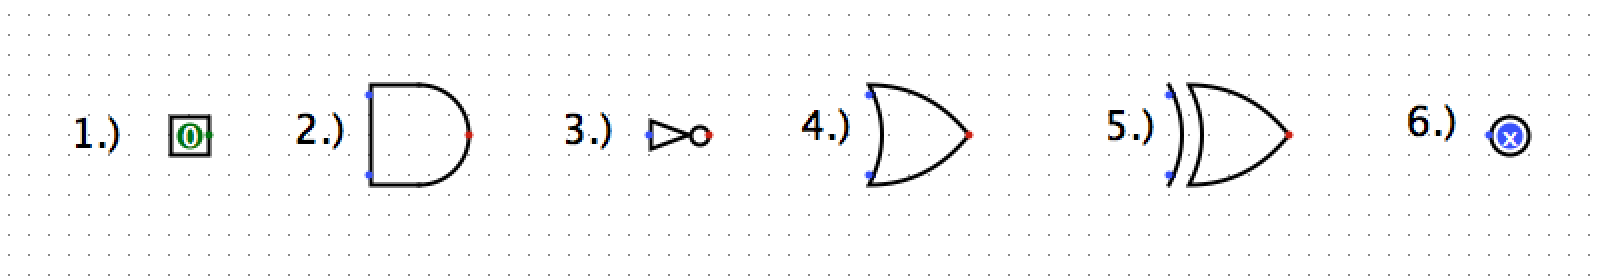
\includegraphics[scale = .35]{logisimgates}
   \caption{Logisim gates for: 1.) inputs 2.) AND gates 3.) NOT gates 4.) OR gates 5.) XOR gates and 6.) output }
   \label{subd}
   \end{figure}
   
   \par With Logisim syntax it is easier to show how a cascading comparison circuit can be extended to 4 bits in figure 5.2.
   
      \begin{figure}[htbp]
      \centering
   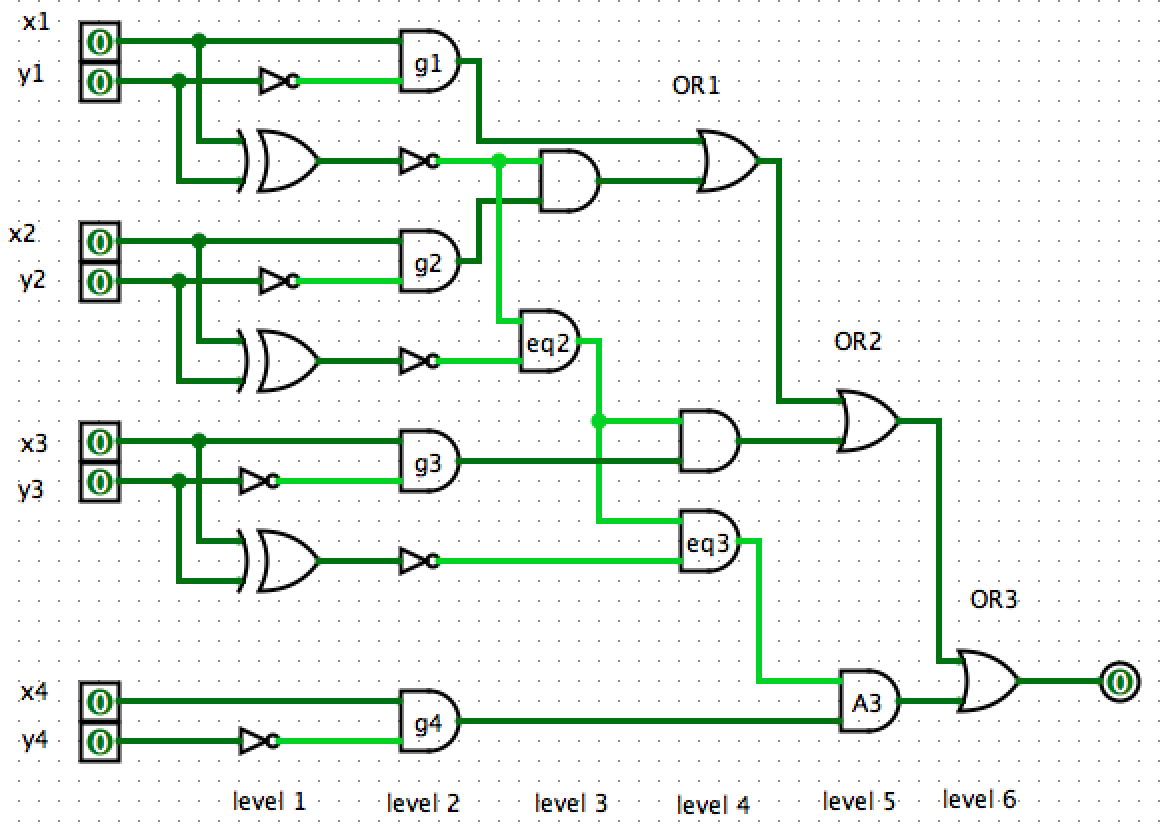
\includegraphics[scale = .55]{comp2_4}
   \caption{4 bit input cascading binary comparison}
   \label{subd}
   \end{figure}
   
   While the syntax may take a little while to get used to, the circuit depicted in figure 5.2  works just as we described with the 2 bit input example, for each bit pair we check if $x_i > y_i$ at the gates labeled ``g$i$", we also check if $x_{\leq i} == y_{\leq i}$ at the gates labeled ``eq$i$''. We describe these circuits with the term \textit{cascading} due to the structure of the gates labeled OR1, OR2, and OR3. 
   \par Consider if we added one more bit of input so it was a 5 bit input comparison circuit as shown in figure 5.3.
 
   \begin{figure}[htbp]
	% the options are h = here, t = top, b = bottom, p = page of figures.
	% you can add an exclamation mark to make it try harder, and multiple
	% options if you have an order of preference, e.g.
	% \begin{figure}[h!tbp]
	   
	       \centering
	    % DO NOT ADD A FILENAME EXTENSION TO THE GRAPHIC FILE
	   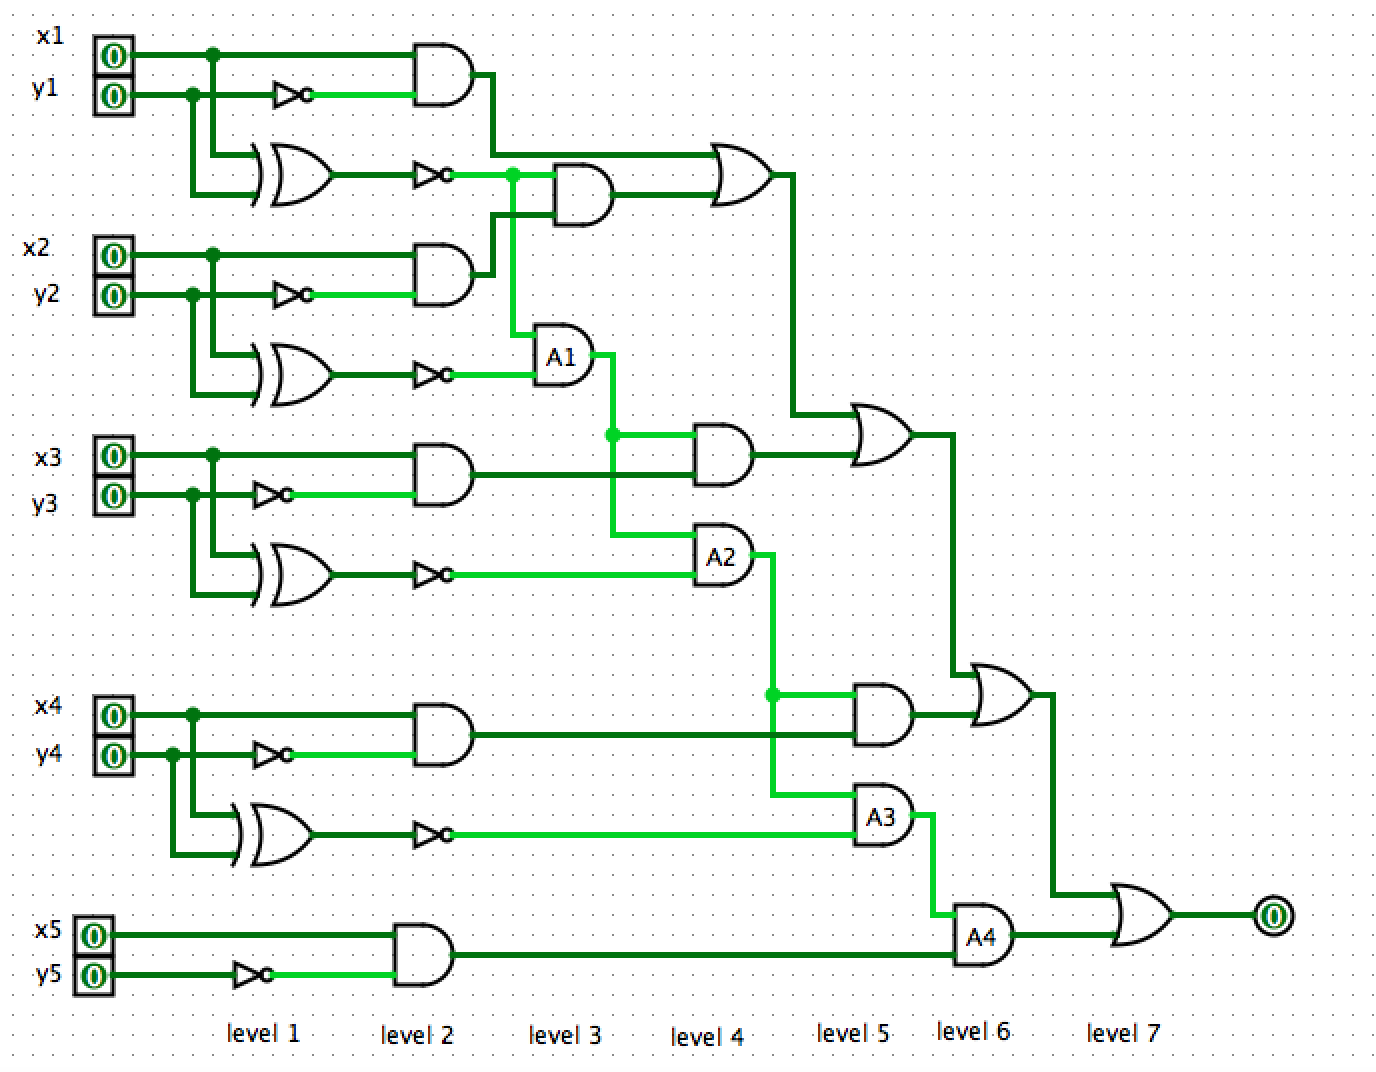
\includegraphics[scale = .5]{comp2_5}
	     \caption{5 bit input cascading binary comparison}
	 \label{subd}
	\end{figure}
	
Notice that in the 4 bit input cascading comparison circuit, the maximum number of AND gates between an input and an output is 3, (eq2, eq3, A3 in figure 5.2), in the 5 bit input cascading comparison circuit the maximum is 4 (A1, A2, A3, A4 as in figure 5.3). If we were to continue to extend the circuit to $n$ input bits, we would see that adding a bit to the input size increases the number of AND gates by 1, this indicates a linear relationship between number of AND gates (remember AND is the same as MUL) and input size. 
 
 \subsection{Chunked Comparison Circuits}
 \par While linear growth of circuits is not horrible, it is reasonable to try to optimize the circuit to a shallower depth to speed up obfuscation. In an attempt to optimize comparison circuits for obfuscation we use the cascading comparison for constant sized chunks of inputs, and then recursively compare these chunks to yield a comparison circuit for arbitrary input length. Rather than the cascading structure of checking $(x_i> y_i) \AND (x_{<i} == y_{<i})$ we try a recursive approach. 
 \par Given two lists of input bits $ x =[x_0,x_1, \cdots x_n], \; y= [y_0,y_1,\cdots , y_n]$ and a chunk size ``cs'',
our recursive chunked comparison circuit generation algorithm runs as follows:
  \begin{itemize}
 \item if $|x|>$cs \textit{ //check if the lists are smaller than the chunk size (we can assume the lists are the same length)}
 	\begin{itemize}
	\item recurse on (the first halves of $x$ and $y$, cs) $\to (g_1,eq_1)$ \textit{//get the values of if $x>y$ and $x==y$ for the first half of the inputs}
	\item recurse on (the second halves of $x$ and $y$, cs) $\to (g_2, eq_2)$ \textit{//get the values of $x>y$ and $x==y$ for the second half of the inputs}
	\item return $(g_1\ \OR\ (eq_1\ \AND\ g_2), \; eq_1\ \AND \ eq_2)$ \textit{// return values of $x>y$ and $x==y$ for this entire chunk}
	\end{itemize} 
\item else run the cascading comparison algorithm on $x$ and $y \to (g,eq)$ \textit{ //return the value of if $(x>y, \; x==y)$ in this chunk}
 \end{itemize}
 
 
 \begin{figure}[htbp]
 	\centering
	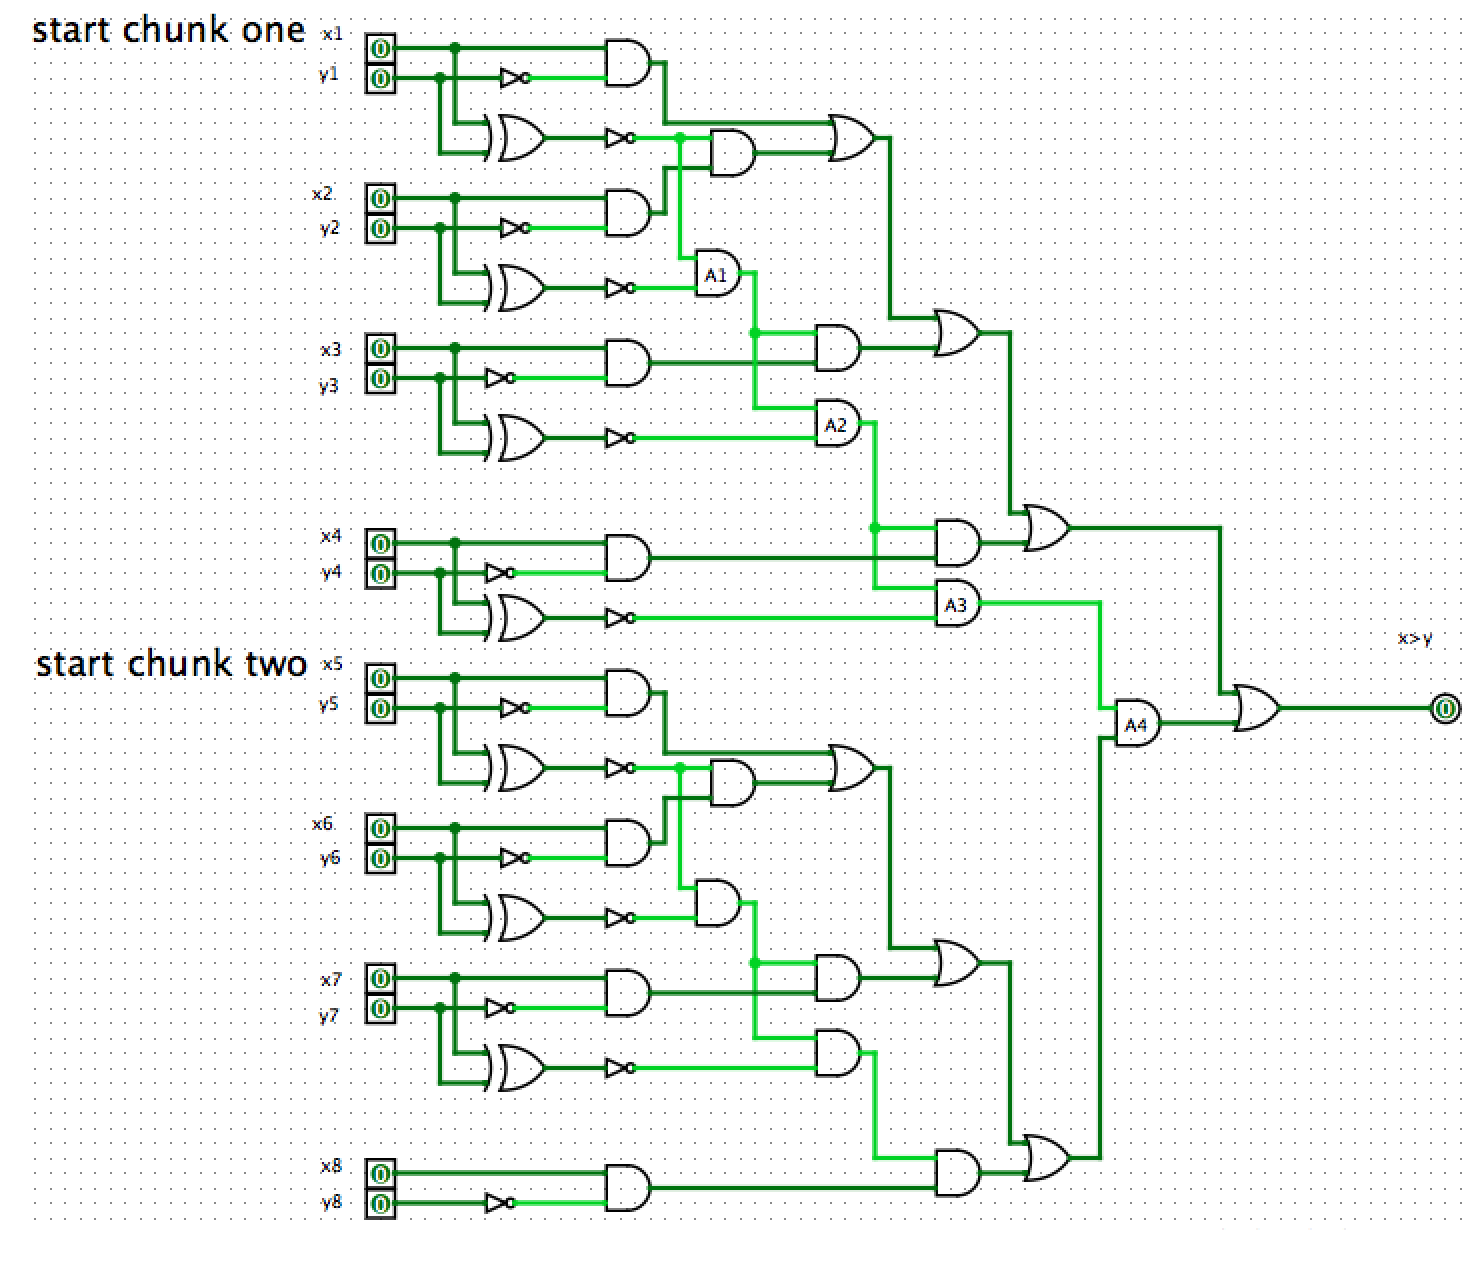
\includegraphics[scale = .6]{ccomp4_8}
	\caption{8 bit input chunked binary comparison}
	\label{subd}
 \end{figure}
 
 \par As you can see in figure 5.4, each chunk is identical to the circuit depicted in figure 5.2, but the equality and greater than values of each chunk are checked at the top level. You can also see that we were able to double the input size of, but still only have a maximum of 4 AND gate from an input to the output (indicated by A1, A2, A3, A4 in figure 5.4). The maximum number of AND gates grows logarithmically as input size increases. We would expect this to mean that chunked comparison is faster to obfuscate than cascading comparison for large input circuits.   
 
 
 \subsection{Multi-Linearity and Efficiency Tests}
 \par We start by testing if reduced circuit depth increases the efficiency of obfuscating the circuit. To test this hypothesis we measure how long it takes to run setup for our two circuit generating algorithms \texttt{comp} (cascading comparison) and \texttt{ccomp8} (chunked comparison with chunk size 8) on circuits with varying input sizes. 
 \begin{table}[htbp] % begins the table floating environment. This enables LaTeX to fit the table where it works best and lets you add a caption.
\caption[]{Efficiency of Chunked and Unchunked Comparison Circuits (Hours: Minutes: Seconds)} 
% The words in square brackets of the caption command end up in the Table of Tables. The words in curly braces are the caption directly over the table.
\begin{center} 
\begin{tabular}{c c c c c c c} 
% the tabular environment is used to make the table itself. The {c c c c} specify that the table will have four columns and they will all be center-aligned. You can make the cell contents left aligned by replacing the Cs with Ls or right aligned by using Rs instead. Add more letters for more columns, and pipes (the vertical line above the backslash) for vertical lines. Another useful type of column is the p{width} column, which forces text to wrap within whatever width you specify e.g. p{1in}. Text will wrap badly in narrow columns though, so beware.
\toprule % a horizontal line, slightly thicker than \hline, depends on the booktabs package
  Total Input Length: &4 &8 &16 &32 &64 &128 \\ % the first row of the table. Separate columns with ampersands and end the line with two backslashes. An environment begun in one cell will not carry over to adjacent rows.
  \midrule % another horizontal line
	\texttt{comp} &00:18:56 &00:44:30 &01:03:37 & 02:38:05 & 06:05:42 &19:54:50\\
	%\texttt{ccomp4} &00:00:01 &00:00:07 &00:04:38 & -- \\
	\texttt{ccomp8} &00:18:35 &11:43:57 &01:03:18 &03:39:36 &11:51:58 & 42:32:49 \\
		\bottomrule % yet another horizontal line
\end{tabular}
\end{center}
\label{inheritance} % labels are useful when you have more than one table or figure in your document. See our online documentation for more on this.
\end{table}

\par As we can see in Table 5.1, \texttt{ccomp8} is about twice as inefficient as \texttt{comp}. Why could this be? While the depth of \texttt{ccomp8} might be shallower than \texttt{comp}, perhaps its multi-linearity (hence forth referred to as $k$) is higher resulting in the setup algorithm needing to find more large primes (as mentioned in section 5.1.1), which is a very expensive computation. 

\par In order to test the multilinearity of our circuits we use the \texttt{get-kappa} setting of \texttt{mio mife} that computes the multi-linearity of our circuits. As we can see in table 5.2 the $k$ values of \texttt{ccomp8} are higher than the corresponding $k$ values of \texttt{comp} by a factor of 2. 
\par At first this was confusing for us, after all, chunking reduces the depth of our circuit and eliminates a lot of AND gates that occur in series in the cascading comparison circuit. However, it's important to remember that $k$ is not just the maximum number of AND (binary MUL) operations in our computation since multiplying a level $i$ and a level $j$ encoding under a graded encoding scheme yields a level $i+j$ encoding. Thus reducing the depth of a circuit does not necessarily make it more efficient to obfuscate.
\par It is also worth noting that the obfuscation scheme itself increases the $k$ value of the obfuscated circuit. While the inner workings of the CMR MIFE scheme [\cite{5genc}] are outside the scope of this thesis, it suffices to say that the $k$ value of a circuit serves as a lower bound on the $k$ value of the obfuscation, so it is more complicated than just tracking the encoding levels from input to output of a circuit.
\par While it is unclear if the relationship between multi-linearity and setup time is causal or not, figure 5.5 shows what looks like a positive linear relationship between them where the slope of the best fit line is approximately 8 minutes as $k$ increase by 1. This constant blow up is the major limitation in obfuscation and functional encryption today since it makes any sort of significant computation infeasible. However, encryption and decryption remain reasonable, for instance \texttt{comp} had a setup time of just over 6 hours, but decryption only took 19 minutes. 

  \begin{figure}[htbp]
	% the options are h = here, t = top, b = bottom, p = page of figures.
	% you can add an exclamation mark to make it try harder, and multiple
	% options if you have an order of preference, e.g.
	% \begin{figure}[h!tbp]
	   
	       \centering
	    % DO NOT ADD A FILENAME EXTENSION TO THE GRAPHIC FILE
	   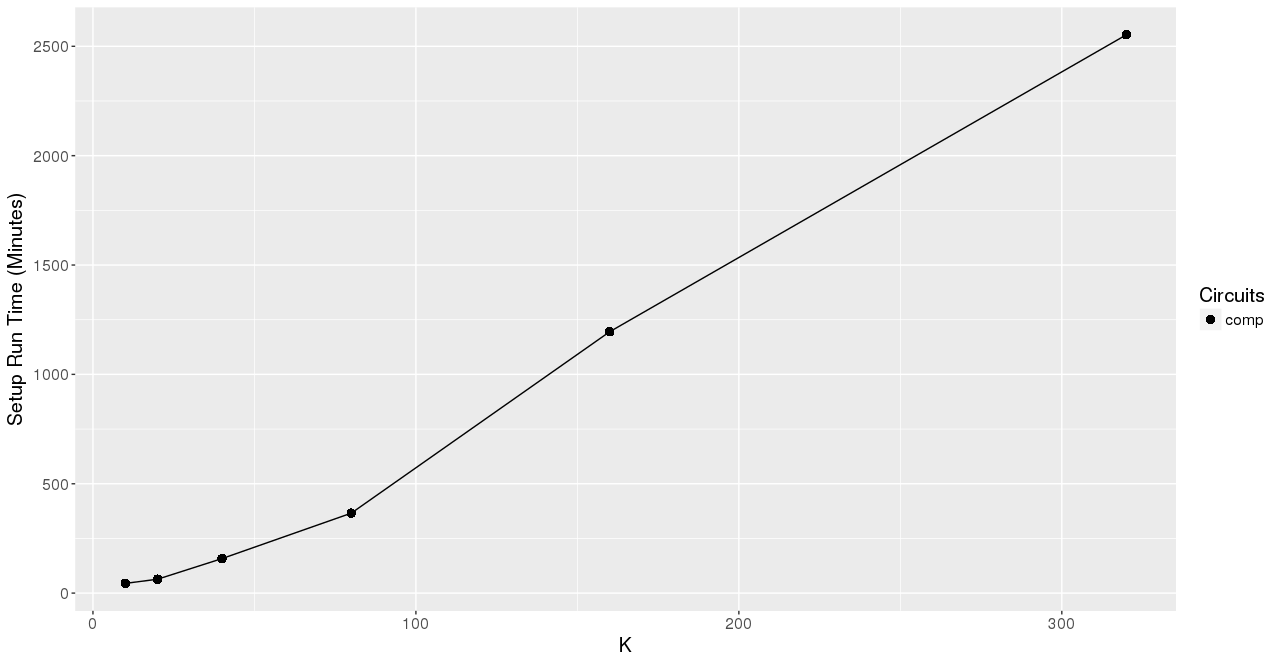
\includegraphics[scale = .46]{SRTvK}
	     \caption{Setup Run Time (Minutes) vs K for \texttt{comp}}
	 \label{subd}
	\end{figure}
 
  
 
 \begin{table}[h] % begins the table floating environment. This enables LaTeX to fit the table where it works best and lets you add a caption.
\caption[Multilinearity of Different Comparison Circuits]{Multilinearity of Chunked and Unchunked Comparison Circuits} 
% The words in square brackets of the caption command end up in the Table of Tables. The words in curly braces are the caption directly over the table.
\begin{center} 
\begin{tabular}{c c c c c c c} 
% the tabular environment is used to make the table itself. The {c c c c} specify that the table will have four columns and they will all be center-aligned. You can make the cell contents left aligned by replacing the Cs with Ls or right aligned by using Rs instead. Add more letters for more columns, and pipes (the vertical line above the backslash) for vertical lines. Another useful type of column is the p{width} column, which forces text to wrap within whatever width you specify e.g. p{1in}. Text will wrap badly in narrow columns though, so beware.
\toprule % a horizontal line, slightly thicker than \hline, depends on the booktabs package
  input lengths: &4 &8 & 16 & 32 &64 &128\\ % the first row of the table. Separate columns with ampersands and end the line with two backslashes. An environment begun in one cell will not carry over to adjacent rows.
  \midrule % another horizontal line
	\texttt{comp} &10 &20 &40 &80 &160 &320\\
	%\texttt{ccomp4} &59 &158 &397 &956 \\
	\texttt{ccomp8} &10 &20 &40 &119 &318 &797\\
		\bottomrule % yet another horizontal line
\end{tabular}
\end{center}
\label{inheritance} % labels are useful when you have more than one table or figure in your document. See our online documentation for more on this.
\end{table}





\subsection{Conclusion}
\par In conclusion, functional encryption is in the early stages of implementation. Right now, functional encryption is limited by the large constant blow up of setup run time related to the increase in the linearity of the circuit. We have also briefly discussed that decryption can be done rather efficiently. As a result, protocols like the online sealed bid first price auction described in section 4.3.2 is feasible so long as the Auction Coordinator has enough processing power to run setup, since decryption is efficient enough for most computers. 



 \bibliographystyle{APA/apa-good}  % or
 \bibliography{thesis}
 % Comment the above two lines and uncomment the next line to use biblatex-chicago.
 %\printbibliography[heading=bibintoc]


\end{document}
